% =====================================================================
% Non-Extensive Entropy Pooling. Working paper (English)
% Compile: pdflatex paper_en.tex  (twice, for references)
% Tables and in-text numbers are generated by paper/build_tables.py
% from the files in results/ (see reproduce_paper.py).
% =====================================================================
\documentclass[11pt]{article}

\usepackage[T1]{fontenc}
\usepackage[utf8]{inputenc}
\usepackage{lmodern}
\usepackage{microtype}
\usepackage[margin=1.1in]{geometry}
\usepackage{amsmath,amssymb,amsthm}
\usepackage{booktabs}
\usepackage{graphicx}
\usepackage{setspace}
\usepackage[round]{natbib}
\usepackage[hidelinks]{hyperref}
\usepackage{caption}
\captionsetup{font=small,labelfont=bf}
\hypersetup{
  pdftitle={Non-Extensive Entropy Pooling: Integrating the Portfolio Manager's Views into Non-Gaussian Markets},
  pdfauthor={Rodrigo Corval\'an Salguero},
  pdfkeywords={entropy pooling, Tsallis entropy, power divergence, effective number of scenarios, Black-Litterman, portfolio choice}
}

\newtheorem{proposition}{Proposition}
\newtheorem{remark}{Remark}

\newcommand{\p}{\mathbf{p}}
\newcommand{\pt}{\tilde{\mathbf{p}}}
\newcommand{\x}{\mathbf{x}}
\newcommand{\R}{\mathbb{R}}
\newcommand{\E}{\mathbb{E}}
\newcommand{\norm}[1]{\left\lVert #1 \right\rVert}

% Generado por paper/build_tables.py. No editar a mano.
\newcommand{\nActiveEq}{8}
\newcommand{\nBootBLdiff}{+0.23}
\newcommand{\nBootBLhi}{+0.99}
\newcommand{\nBootBLlo}{-0.38}
\newcommand{\nBootEPdiff}{+0.02}
\newcommand{\nBootEPeqdiff}{+0.13}
\newcommand{\nBootEPeqhi}{+0.59}
\newcommand{\nBootEPeqlo}{-0.26}
\newcommand{\nBootEPhi}{+0.14}
\newcommand{\nBootEPlo}{-0.13}
\newcommand{\nBootPriorLoMax}{+0.09}
\newcommand{\nBootPriorLoMin}{-0.08}
\newcommand{\nBootPriordiff}{+1.21}
\newcommand{\nBootPriorhi}{+2.89}
\newcommand{\nBootPriorlo}{+0.01}
\newcommand{\nBootReps}{500}
\newcommand{\nBootSdSFifty}{42.5}
\newcommand{\nBootSdSTwenty}{8.3}
\newcommand{\nBootSdTFifty}{10.2}
\newcommand{\nBootSdTTwenty}{4.8}
\newcommand{\nBootUsualdiff}{+0.99}
\newcommand{\nBootUsualhi}{+2.33}
\newcommand{\nBootUsuallo}{-0.08}
\newcommand{\nCVaRSFifty}{-4.11}
\newcommand{\nCVaRSFive}{-6.90}
\newcommand{\nCVaRSTwenty}{-5.38}
\newcommand{\nCVaRTFifty}{0.05}
\newcommand{\nCVaRTFive}{-6.67}
\newcommand{\nCVaRTTwenty}{-3.86}
\newcommand{\nCVaRprior}{-7.91}
\newcommand{\nContribTop}{38.6}
\newcommand{\nContribTotal}{18.9}
\newcommand{\nCostEP}{0.6}
\newcommand{\nDays}{121}
\newcommand{\nDwFifty}{1.18}
\newcommand{\nDwFive}{0.08}
\newcommand{\nDwTwenty}{0.29}
\newcommand{\nEnsSFifty}{0.595}
\newcommand{\nEnsSFive}{0.993}
\newcommand{\nEnsSTwenty}{0.903}
\newcommand{\nEnsTFifty}{0.449}
\newcommand{\nEnsTFive}{0.993}
\newcommand{\nEnsTTwenty}{0.884}
\newcommand{\nEssEq}{99.97}
\newcommand{\nEssHist}{99.99}
\newcommand{\nExFifty}{1098}
\newcommand{\nExFive}{110}
\newcommand{\nExTwenty}{439}
\newcommand{\nExtBench}{21.7}
\newcommand{\nExtDay}{27~October~2025}
\newcommand{\nExtMVhist}{14.4}
\newcommand{\nImprovPct}{0.21}
\newcommand{\nIneq}{11}
\newcommand{\nJ}{1906}
\newcommand{\nKishSFifty}{0.116}
\newcommand{\nKishSFiftyPct}{12}
\newcommand{\nKishSFive}{0.987}
\newcommand{\nKishSTwenty}{0.755}
\newcommand{\nKishTFifty}{0.361}
\newcommand{\nKishTFiftyPct}{36}
\newcommand{\nKishTFive}{0.987}
\newcommand{\nKishTTwenty}{0.815}
\newcommand{\nLimA}{5.3\times 10^{-6}}
\newcommand{\nLimB}{5.4\times 10^{-7}}
\newcommand{\nLimC}{5.4\times 10^{-8}}
\newcommand{\nLoneBLeq}{0.54}
\newcommand{\nLoneBLhist}{0.38}
\newcommand{\nLoneEPeq}{0.36}
\newcommand{\nLoneEPeqFull}{0.67}
\newcommand{\nLoneEPhist}{0.15}
\newcommand{\nLonePrior}{1.30}
\newcommand{\nLoneQeq}{0.003}
\newcommand{\nLoneQhist}{0.0002}
\newcommand{\nMaxSFifty}{113}
\newcommand{\nMaxSFive}{2.2}
\newcommand{\nMaxSTwenty}{15.9}
\newcommand{\nMaxTFifty}{13.7}
\newcommand{\nMaxTFive}{1.8}
\newcommand{\nMaxTTwenty}{4.5}
\newcommand{\nMeucciN}{10}
\newcommand{\nMuHistMax}{79}
\newcommand{\nMuHistMin}{55}
\newcommand{\nN}{20}
\newcommand{\nOctaveDiff}{$2\times 10^{-6}$}
\newcommand{\nPiBankMax}{70}
\newcommand{\nPiBankMin}{66}
\newcommand{\nPiLowMax}{42}
\newcommand{\nPiLowMin}{35}
\newcommand{\nQtwoErr}{0.045944}
\newcommand{\nRankDw}{0.001}
\newcommand{\nRankEss}{0.998}
\newcommand{\nRetBL}{48.1}
\newcommand{\nRetBLhist}{68.7}
\newcommand{\nRetBench}{49.0}
\newcommand{\nRetEP}{67.2}
\newcommand{\nRetEPeq}{47.6}
\newcommand{\nRetEW}{53.8}
\newcommand{\nRetMVhist}{67.9}
\newcommand{\nRetMinVar}{62.7}
\newcommand{\nRobEqMax}{+0.24}
\newcommand{\nRobMax}{+0.06}
\newcommand{\nRobMin}{-0.06}
\newcommand{\nRobQmax}{0.003}
\newcommand{\nRobQmaxEq}{0.02}
\newcommand{\nSEann}{22}
\newcommand{\nSEday}{0.087}
\newcommand{\nShBL}{2.20}
\newcommand{\nShBLhist}{3.24}
\newcommand{\nShBench}{1.97}
\newcommand{\nShBenchDaily}{2.06}
\newcommand{\nShBenchEx}{1.35}
\newcommand{\nShBenchRf}{1.42}
\newcommand{\nShEP}{3.19}
\newcommand{\nShEPeq}{2.10}
\newcommand{\nShEW}{2.04}
\newcommand{\nShMVhist}{3.18}
\newcommand{\nShMVhistEx}{2.85}
\newcommand{\nShMVhistRf}{2.45}
\newcommand{\nShMinVar}{2.81}
\newcommand{\nShPlaceboEP}{3.24}
\newcommand{\nShPlaceboEPeq}{1.97}
\newcommand{\nShWinNVmax}{2.15}
\newcommand{\nShWinNVmin}{2.07}
\newcommand{\nShannonErr}{0.046040}
\newcommand{\nShannonShift}{3.5\times 10^{-4}}
\newcommand{\nShiftEq}{12}
\newcommand{\nTurnEP}{116\%}
\newcommand{\nVolKishSThree}{0.166}
\newcommand{\nVolKishSTwo}{0.615}
\newcommand{\nVolKishTThree}{0.201}
\newcommand{\nVolKishTTwo}{0.642}
\newcommand{\nWIlliq}{59}
\newcommand{\nZeroIlliqMax}{4.1}
\newcommand{\nZeroIlliqMin}{3.2}
\newcommand{\nZeroLiqMax}{1.4}
\newcommand{\nZeroLiqMin}{0.5}
\newcommand{\nZerosFifty}{734}
\newcommand{\nZerosFiftyPct}{39}
\newcommand{\nZerosFive}{1}
\newcommand{\nZerosTwenty}{39}


\title{\textbf{Non-Extensive Entropy Pooling:\\ Integrating the Portfolio Manager's Views\\ into Non-Gaussian Markets}\thanks{The author thanks \'Alvaro Corval\'an, PhD, for his review of the sections on the generalization of entropy, and Pablo J.~Escapa for sharing the equity views used in Section~\ref{sec:empirical}. The opinions expressed are the author's and do not necessarily reflect those of the institutions with which he is affiliated or of the persons acknowledged. This paper is not investment advice. The availability of code and data and the other statements are in the Declarations section. All errors are the author's. Comments are welcome.}}

\author{Rodrigo Corval\'an Salguero\\ \small Universidad Torcuato Di Tella\\ \small Universidad de Buenos Aires\\ \small \texttt{rodrigocorvalan93@gmail.com}}
\date{This version: November 2026}

\begin{document}
\maketitle

\begin{abstract}
\noindent
Entropy Pooling \citep{Meucci2008} updates a scenario-based market prior
with a portfolio manager's views by minimizing the Kullback--Leibler
divergence subject to the views, written as linear constraints on the
scenario probabilities. This paper replaces that divergence with the Tsallis
relative entropy of order $q$ and gives the posterior for $q>1$ in closed form up to the multipliers of a
concave dual problem. With a uniform prior, the posterior of order $q$ maximizes the
effective number of scenarios of the same order: classical Entropy Pooling
maximizes the entropy-based measure of \citet{Meucci2012}, and $q=2$
maximizes the effective sample size of \citet{Kish1965} and equals the
Euclidean projection of the prior onto the set of distributions that satisfy
the views. Two further results limit the cases in which the choice matters: all members
of the family agree to first order in the size of the views, and they
coincide exactly for views on the probability of an event. A stress
experiment on Argentine equities shows the trade-off for demanding views on
means. For a view fifty standard errors away from the sample mean, the $q=2$
posterior has a Kish effective sample size of \nKishTFiftyPct\% of the
number of scenarios, against \nKishSFiftyPct\% for classical Entropy
Pooling, but it assigns zero probability
to \nZerosFiftyPct\% of the scenarios and removes the adverse tail of the
stressed stock. In an application with a practitioner's views the choice of
$q$ is immaterial. A design that crosses two priors with three updating
rules shows that the out-of-sample gap between Entropy Pooling and
Black--Litterman in their usual configurations is the gap between their
priors, and that in a window of six months no difference between the
portfolios is clearly distinguishable from zero.
\medskip

\noindent\textbf{Keywords:} entropy pooling; Tsallis entropy; power
divergence; effective number of scenarios; Black--Litterman; portfolio
choice.\\
\textbf{JEL codes:} G11, C61, C11.
\medskip

\noindent\textbf{AI disclosure:} the author used Claude (Anthropic) to
review the model, the code and the literature, derive the propositions of
Section~\ref{sec:optimalq}, implement the stress experiment and the
robustness checks, and draft the text. The author is responsible for the
content.
\end{abstract}

\onehalfspacing

% ---------------------------------------------------------------------
\section{Introduction}
% ---------------------------------------------------------------------

Portfolio construction combines a statistical description of the market,
the prior, with the judgment of the portfolio manager, the views. In
the model of \citet{BlackLitterman1992} the prior is a normal distribution
centred at the returns implied by market equilibrium
\citep{HeLitterman2002}, the views are noisy linear statements about
expected returns, and the posterior is again normal. The model is tractable,
but a view about a ranking, a volatility or a tail cannot be stated in it,
and the posterior keeps the shape of the prior.

\citet{Meucci2008} proposed updating probabilities instead of parameters.
In Entropy Pooling (EP) the prior is a set of $J$ scenarios with
probabilities $\p$, a view is a linear constraint on those probabilities,
and the posterior is the distribution closest to the prior in relative
entropy among those that satisfy the views. Any statement that is linear in
the probabilities can be a view, including inequalities between expected
returns and bounds on tail probabilities, and the scenarios keep whatever
skewness, kurtosis and dependence they have. This is the sense in which the
approach is suited to non-Gaussian markets: the non-normality is in the
scenarios, and the update does not remove it.

Relative entropy is one of many divergences. It is the limit, as $q \to 1$,
of the relative entropy associated with the entropy of \citet{Tsallis1988}
\citep{BorlandPlastinoTsallis1998}, a one-parameter family that arose in
non-extensive statistical mechanics \citep{Tsallis2009} and that coincides,
up to a constant factor, with the power divergences of
\citet{CressieRead1984}. This paper studies Entropy Pooling under that
family: how the posterior is computed, what the parameter $q$ controls, and
when its value matters for a portfolio.

First, the paper writes the problem and its dual in
the scenario setting of EP, with equality and inequality views: for $q>1$
the posterior probability of a scenario is a truncated power of a linear
combination of the view functions evaluated at that scenario, and it is
found by solving a concave dual problem with one variable per
view (Section~\ref{sec:framework}). Second, with a uniform prior the posterior of
order $q$ maximizes the effective number of scenarios of order $q$
(Proposition~\ref{prop:hill}). Classical EP therefore maximizes the
entropy-based effective number of scenarios that \citet{Meucci2012}
proposed as a diagnostic for EP, and $q=2$ maximizes the effective sample
size of \citet{Kish1965}; the $q=2$ posterior is also the Euclidean
projection of the prior onto the set of distributions that satisfy the
views. Each member of the family is thus optimal for its own measure, and a
numerical search over $q$ scored by Euclidean distance has to return $q=2$.
Third, the members of the family differ less than this might suggest. They
agree to first order in the size of the views
(Proposition~\ref{prop:local}) and they coincide exactly when the views fix
the probabilities of the cells of a partition, as a tail view on one asset
does (Proposition~\ref{prop:jeffrey}). The parameter matters for demanding views
on moments. A stress experiment on Argentine equities
(Section~\ref{sec:separation}) quantifies the trade-off in that case: the
$q=2$ posterior spreads probability more evenly over the scenarios it
keeps, and the posterior of classical EP, called the Shannon posterior
below, keeps all the scenarios.

Fourth, an application to the leading panel of the Buenos Aires stock
exchange uses the ranking and relative views of a practitioner
(Section~\ref{sec:empirical}). These views ask for a small change of the prior, and
EP and its $q=2$ version give the same portfolio. The application is
designed to separate the prior from the updating rule. Black--Litterman
starts from equilibrium returns and EP from historical scenarios, so a
direct comparison of the two confounds the prior with the updating rule.
The design crosses two priors (equilibrium and historical) with three
updating rules (Black--Litterman, EP and EP with $q=2$) and adds a
portfolio without views for each prior. Over the six months that follow
the formation date, the gap between EP and Black--Litterman in their usual
configurations is the gap between the two no-view portfolios, that is,
between the priors. Within each prior the views change the out-of-sample
Sharpe ratio by amounts that cannot be distinguished from zero, and the
difference between the priors is itself at the margin of what a window of
that length can detect.

None of the mathematics is new; Section~\ref{sec:literature} places it in
the literature. The closest antecedent in finance is \citet{DeyJuneja2012},
who incorporate views by minimizing a divergence equivalent to the relative
entropies of Tsallis and R\'enyi. What this paper adds is the treatment of
the scenario-probability problem of EP with inequality views, the
characterization of each member of the family by its effective number of
scenarios, an assessment of when the choice of member matters, and an
application.

The code that produces every table and figure is public; see the
Declarations section.

% ---------------------------------------------------------------------
\section{Related literature}\label{sec:literature}
% ---------------------------------------------------------------------

Entropy Pooling belongs to a long line of work on updating by minimum
divergence. \citet{Kullback1959} introduced the principle of minimum
discrimination information and \citet{Csiszar1975} gave its geometry. In
finance the same projection reweights scenarios in the canonical valuation
of \citet{Stutzer1996} and in the weighted Monte Carlo method of
\citet{AvellanedaEtAl2001}, and \citet{Pezier2007} proposed it as an
alternative to Black--Litterman shortly before \citet{Meucci2008} gave the
formulation in terms of scenario probabilities that is used here.
\citet{Meucci2012} added the effective number of scenarios as a diagnostic
of the posterior.

Replacing the Kullback--Leibler divergence by a power divergence is common
in statistics and econometrics. The Tsallis relative entropy of order $q$
is, up to a constant factor, the power divergence of
\citet{CressieRead1984} with index $\lambda = q-1$, and the divergence of
\citet{Renyi1961} is a monotone transformation of it. The probabilities
that minimize a member of this family subject to moment conditions are the
implied probabilities of generalized empirical likelihood
\citep{NeweySmith2004}: $q \to 1$ is exponential tilting
\citep{KitamuraStutzer1997,ImbensSpadyJohnson1998} and $q=2$ is the
Euclidean likelihood, whose implied probabilities are linear in the moment
functions \citep{AntoineBonnalRenault2007}. In survey sampling the same two
cases are the raking and the linear methods of calibration of
\citet{DevilleSarndal1992}, who show that all the estimators of the family
are asymptotically equivalent; \citet{GlassermanYu2005} prove the
corresponding result for weighted Monte Carlo. The dual problem of
Section~\ref{sec:dual} is the standard dual of a convex divergence
minimized under linear constraints \citep{BorweinLewis1991}.

In finance, \citet{DeyJuneja2012} study the incorporation of views by
minimum divergence with explicit reference to Entropy Pooling. They show
that the Kullback--Leibler solution may not exist when the prior has fat
tails, and use a polynomial divergence that is an increasing function
of the relative entropies of Tsallis and R\'enyi; their setting is a
continuous model with constraints on moments and on marginal
distributions. Other members of the family have been used to assess asset
pricing models \citep{AlmeidaGarcia2012} and to measure model risk with
heavy tails \citep{GlassermanXu2014}.
\citet{MakamMillossovichTsanakas2021} stress simulated scenarios by
minimizing the $\chi^2$ divergence and find a lower sampling error than
with the Kullback--Leibler divergence, which is consistent with the
results of Section~\ref{sec:separation}.

The relation between the $\chi^2$ divergence, the Euclidean distance to
uniform weights and the effective sample size is also classical. The
quantity $1/\sum_j x_j^2$ is the effective sample size associated with the
design effect of \citet{Kish1965}; it entered importance sampling with
\citet{KongLiuWong1994}. Weights that minimize their own variance subject
to moment constraints, and therefore maximize this effective sample size,
are the stable weights of \citet{Zubizarreta2015}. The Kish number and the
entropy-based number of \citet{Meucci2012} belong to the family of
effective numbers of \citet{Hill1973}, with orders 2 and 1 respectively.

Which divergence should be used for inference under linear constraints is
an old question. \citet{ShoreJohnson1980} derive the Kullback--Leibler
divergence from consistency axioms, and \citet{Csiszar1991} characterizes
least squares and minimum discrimination information, which are the
members $q=2$ and $q \to 1$ compared in this paper, as the two rules
singled out by natural postulates. The use of non-additive entropies for
inference has been criticized \citep{PresseEtAl2013} and defended
\citep{Tsallis2015,JizbaKorbel2019}. This paper takes no position in that
debate: the family is used as a one-parameter set of divergences, and the
arguments for one member or another rest on the shape of the reweighting
and on the sampling variance of posterior estimates, not on
non-extensivity. One property is lost when $q \ne 1$: if the prior is a
product of two independent blocks and each view involves one block, the
Shannon posterior is the product of the posteriors of the blocks, and the
posterior of order $q \ne 1$ is not. Tsallis statistics has also been applied to the
distribution of asset returns and to option pricing
\citep{Borland2002,TsallisEtAl2003}, which is a different use from the
reweighting of scenarios considered here.

Relative to this literature the contribution is applied. To the author's
knowledge, the power-divergence family has not been taken to the
scenario-probability problem of Entropy Pooling with equality and
inequality views.

% ---------------------------------------------------------------------
\section{Entropy Pooling with a Tsallis divergence}\label{sec:framework}
% ---------------------------------------------------------------------

\subsection{Prior, views and the problem}

Let $X \in \R^{J \times N}$ be a panel of $J$ scenarios for $N$ assets.
The scenarios can be historical returns, simulated paths or any other
representation of the market invariants, the variables whose distribution
is taken to be stable over time. Let $\p$ be the prior
probabilities of the scenarios, with $p_j > 0$ and $\sum_j p_j = 1$; in
most applications the prior is uniform, $p_j = 1/J$. The views are linear
constraints on the posterior probabilities $\x$:
\begin{equation}\label{eq:constraints}
A\x \le \mathbf{b}, \qquad A_{eq}\x = \mathbf{b}_{eq},
\end{equation}
where the rows of $A$ and $A_{eq}$ are functions of the scenarios. A row
equal to the returns of asset $i$ imposes a value or a bound on its
expected return; the difference of two such rows imposes a ranking,
$\E[X_i] \ge \E[X_k]$; squared returns give views on second moments; and
the indicator of an event gives a view on its probability, for example
$\sum_{j:\,X_{ji} < t} x_j \le \pi$ for a tail. The normalization
$\mathbf{1}^\top \x = 1$ is one of the equality rows. The set of
distributions that satisfy the views is
\begin{equation}\label{eq:feasible}
\mathcal{F} = \{\x \ge 0 : A\x \le \mathbf{b},\; A_{eq}\x = \mathbf{b}_{eq}\},
\end{equation}
and it is assumed to be non-empty.

The posterior is the element of $\mathcal{F}$ closest to the prior,
\begin{equation}\label{eq:primal}
\pt \;=\; \arg\min_{\x \in \mathcal{F}} \; D(\x \,\|\, \p),
\end{equation}
for a divergence $D$. Classical EP uses the Kullback--Leibler divergence,
\[
D_{KL}(\x\|\p) = \sum_j x_j \ln \frac{x_j}{p_j}.
\]

\subsection{The Tsallis family}

For $q > 0$, $q \neq 1$, the Tsallis relative entropy of order $q$ is
\begin{equation}\label{eq:tsallis}
D_q(\x \,\|\, \p) \;=\; \frac{1}{q-1}\left( \sum_{j=1}^{J} \frac{x_j^{\,q}}{p_j^{\,q-1}} - 1 \right),
\end{equation}
and $D_q \to D_{KL}$ as $q\to 1$ (Appendix~\ref{app:proofs}). The power
divergence of \citet{CressieRead1984} with index $\lambda$ is proportional
to $D_q$ with $q = \lambda + 1$ (it equals $D_q/q$), so the two families
have the same
minimizers. For $q=2$, $D_2(\x\|\p) = \sum_j (x_j-p_j)^2/p_j$ is the
Pearson $\chi^2$ divergence. For every $q>0$ the function
$\x \mapsto D_q(\x\|\p)$ is strictly convex on the simplex, so
problem~\eqref{eq:primal} has a unique solution.

\subsection{Dual solution}\label{sec:dual}

Let $\boldsymbol{\lambda} \ge 0$ be the multipliers of the inequalities and
$\boldsymbol{\nu}$ those of the equalities, and write
$\mathbf{z} = A^\top \boldsymbol{\lambda} + A_{eq}^\top \boldsymbol{\nu}$.
Minimizing the Lagrangian over $\x \ge 0$ gives the posterior as a function
of the multipliers:
\begin{align}
\text{Shannon } (q \to 1): \quad & x_j \;=\; p_j \exp\!\big( - 1 - z_j \big), \label{eq:kkt-shannon}\\[2pt]
\text{Tsallis } (q > 1): \quad & x_j \;=\; p_j \,\Big[ \max\!\Big( -\frac{q-1}{q}\, z_j,\; 0 \Big) \Big]^{\frac{1}{q-1}}. \label{eq:kkt-tsallis}
\end{align}
The Shannon posterior tilts the prior exponentially and gives positive
probability to every scenario. The Tsallis posterior tilts it by a power
of a linear combination of the view functions evaluated at the scenario,
and assigns probability zero to the scenarios in which that combination is
not positive. The zero is part of the
solution: when $z_j \ge 0$ the Lagrangian increases with $x_j$ and its
minimum over $x_j \ge 0$ is at $x_j = 0$ (Appendix~\ref{app:dual}). For
$q=2$ the tilt is linear and truncated at zero. If the views are equalities, $A_{eq}$ has full row rank
and no probability is truncated, the multipliers of $q=2$ solve a linear
system and the posterior is
$\x = \p + P A_{eq}^\top (A_{eq} P A_{eq}^\top)^{-1}
(\mathbf{b}_{eq} - A_{eq}\p)$, with $P = \mathrm{diag}(\p)$: these are the
weights of linear calibration \citep{DevilleSarndal1992} and the implied
probabilities of the Euclidean likelihood
\citep{AntoineBonnalRenault2007}.

Substituting~\eqref{eq:kkt-shannon} or~\eqref{eq:kkt-tsallis} into the
Lagrangian gives the dual function \citep{BorweinLewis1991}, a concave
function of
$(\boldsymbol{\lambda}, \boldsymbol{\nu})$, to be maximized subject to
$\boldsymbol{\lambda} \ge 0$. Its gradient is the vector of constraint
residuals
$\big(A\x - \mathbf{b},\; A_{eq}\x - \mathbf{b}_{eq}\big)$, and there is no
duality gap when some distribution with positive probabilities satisfies
the views. The dual has one variable per view, whatever the number of
scenarios.
The implementation rescales each constraint by the root mean square of its
row, maximizes the dual with a quasi-Newton method started, for $q>1$, at
the Shannon multipliers, refines the solution with Newton steps on the
optimality conditions, and accepts it only if those conditions hold to a
tolerance of $10^{-8}$ in the rescaled units. With $J = 10^5$ scenarios and
one view, each problem is solved in less than a second.

\subsection{Confidence}

Partial confidence $c \in [0,1]$ in the views follows \citet{Meucci2008}:
the posterior used for portfolio construction is the mixture
$\pt_c = (1-c)\,\p + c\,\pt$. The target of an individual view can also be
moved towards its value under the prior before solving. The two mechanisms
compound, and Section~\ref{sec:empirical} uses only the first.

% ---------------------------------------------------------------------
\section{What the parameter \texorpdfstring{$q$}{q} controls}\label{sec:optimalq}
% ---------------------------------------------------------------------

\subsection{Effective number of scenarios}

A posterior that concentrates probability on a few scenarios uses little
of the sample. The usual summaries of this concentration are effective
numbers of scenarios. For a distribution $\x$ and an order $q>0$,
$q \ne 1$, let
\begin{equation}\label{eq:hill}
N_q(\x) \;=\; \Big( \sum_{j} x_j^{\,q} \Big)^{\frac{1}{1-q}},
\qquad
N_1(\x) \;=\; \lim_{q \to 1} N_q(\x) \;=\; \exp\!\Big( -\sum_j x_j \ln x_j \Big).
\end{equation}
These are the diversity numbers of \citet{Hill1973}. All of them equal $J$
for the uniform distribution and $1$ for a distribution concentrated on one
scenario. $N_1$ is the effective number of scenarios that
\citet{Meucci2012} proposed for Entropy Pooling posteriors, and
$N_2 = 1/\sum_j x_j^2$ is the effective sample size of \citet{Kish1965}.

\begin{proposition}[Effective number of scenarios]\label{prop:hill}
Let the prior be uniform, $p_j = 1/J$, and let $\mathcal{F}$ be the set
in~\eqref{eq:feasible}. Then:
\begin{enumerate}
\item[(i)] for every $q>0$, $q \ne 1$, the posterior
      $\pt_q = \arg\min_{\x \in \mathcal{F}} D_q(\x\|\p)$ maximizes $N_q$
      over $\mathcal{F}$, and the Shannon posterior maximizes $N_1$;
\item[(ii)] the posterior of order $2$ is the Euclidean projection of the
      prior onto $\mathcal{F}$, that is,
      $\pt_2$ minimizes $\norm{\x - \p}_2$ over $\x \in \mathcal{F}$;
\item[(iii)] for every $\x \in \mathcal{F}$,
      $\norm{\x - \p}_2 \ge \norm{\pt_2 - \p}_2$ and
      $N_2(\x) \le N_2(\pt_2)$, with equality only if $\x = \pt_2$.
\end{enumerate}
\end{proposition}

\begin{proof}
Write $S_q(\x) = \sum_j x_j^q$. With $p_j = 1/J$,
$D_q(\x\|\p) = (J^{q-1} S_q(\x) - 1)/(q-1)$ and
$N_q(\x) = S_q(\x)^{1/(1-q)}$. For $q>1$, $D_q$ increases and $N_q$
decreases with $S_q$; for $q<1$, $D_q$ decreases and $N_q$ increases with
$S_q$. In both cases minimizing $D_q$ over $\mathcal{F}$ is maximizing
$N_q$. For the Shannon posterior,
$D_{KL}(\x\|\p) = \ln J + \sum_j x_j \ln x_j = \ln\big(J/N_1(\x)\big)$.
This proves (i). On the simplex,
$\norm{\x-\p}_2^2 = S_2(\x) - 1/J$, an increasing function of $S_2$, which
gives (ii). Part (iii) follows from (i), (ii) and the uniqueness of the
projection onto a closed convex set.
\end{proof}

Proposition~\ref{prop:hill} refers to the posterior with full confidence.
For $c<1$ the statements about the Euclidean distance and $N_2$ carry over
to the mixture $\pt_c$, because
$\norm{\pt_c - \p}_2 = c\,\norm{\pt - \p}_2$; the statement about $N_1$
does not, since the mixture of the Shannon posterior with the prior need
not have the largest $N_1$ among the mixtures.

Proposition~\ref{prop:hill} has two consequences for how $q$ should be
chosen. The first is that a numerical criterion taken from the family
selects its own member. A search over $q$ that scores each posterior by its
Euclidean distance to the prior returns $q=2$ by part (ii), and one that
scores by the entropy-based effective number returns $q \to 1$ by part (i).
Section~\ref{sec:numerics} reports such a search as a check of the
implementation; it is not evidence about which $q$ is preferable.

The second is that the order should be chosen according to the use of
the posterior. If the scenarios are independent draws and $f$ is a function of
the scenario with variance $\sigma_f^2$, the weighted average
$\sum_j x_j f(X_j)$ has variance $\sigma_f^2 \sum_j x_j^2 = \sigma_f^2 /
N_2(\x)$ for given weights. This is the design-effect argument of
\citet{Kish1965}; it is an approximation here because the posterior weights
depend on the scenarios through the views. Posterior means and covariances,
the inputs of a mean--variance optimization, are averages of this kind. By
part (iii), $q=2$ gives, among the distributions that satisfy the views,
the one for which such averages have the smallest sampling variance;
Section~\ref{sec:separation} checks this by resampling the scenarios.
The measure of order 1 has no similar reading, but the posterior that
maximizes it keeps all the scenarios, which matters when the posterior is
used to measure tail risk (Section~\ref{sec:separation}).

With a prior that is not uniform the correspondence is with relative
measures: the $q=2$ posterior minimizes
$\sum_j (x_j - p_j)^2/p_j$, the squared Euclidean distance in the metric of the
prior, and $1/(1+D_2)$ is the ratio of effective to actual sample size used in
importance sampling \citep{KongLiuWong1994}.

\subsection{Two cases in which \texorpdfstring{$q$}{q} does not matter}

The members of the family are closer to each other than their different
functional forms suggest. Write the divergences in the common form
$D_\varphi(\x\|\p) = \sum_j p_j\, \varphi(x_j/p_j)$, with
$\varphi_q(u) = (u^q-1)/(q-1)$ for the Tsallis family and
$\varphi(u) = u \ln u$ for Kullback--Leibler. In all these cases $\varphi$
is strictly convex and smooth around $1$, with $\varphi''(1) = q$ and
$\varphi''(1)=1$ respectively.

\begin{proposition}[First-order equivalence]\label{prop:local}
Consider equality views $A_{eq}\x = A_{eq}\p + \varepsilon\,\mathbf{d}$,
where $A_{eq}$ has full row rank and includes the normalization, the
component of $\mathbf{d}$ in the normalization row is zero, and
$P = \mathrm{diag}(\p)$. For every $\varphi$ that is strictly convex on
$[0,\infty)$ and twice continuously differentiable in a neighbourhood of
$1$ with $\varphi''(1) > 0$, the posterior satisfies
\begin{equation}\label{eq:linear}
\pt_\varphi(\varepsilon) \;=\; \p \;+\; \varepsilon\, P A_{eq}^\top
\big(A_{eq} P A_{eq}^\top\big)^{-1} \mathbf{d} \;+\; o(\varepsilon)
\qquad (\varepsilon \to 0).
\end{equation}
The first-order term does not depend on $\varphi$. In particular
$\norm{\pt_q(\varepsilon) - \pt_{q'}(\varepsilon)} = o(\varepsilon)$ for any
two orders $q$ and $q'$, and the same holds between any order and the
Shannon posterior.
\end{proposition}

The proof is in Appendix~\ref{app:proofs}. The first-order term
of~\eqref{eq:linear} is the $q=2$ solution without the truncation at zero.
With inequality views $A\x \le A\p + \varepsilon\,\mathbf{d}$ the
first-order term is $\varepsilon\,\boldsymbol{\delta}$, where
$\boldsymbol{\delta}$ minimizes $\sum_j \delta_j^2/p_j$ subject to
$A\boldsymbol{\delta} \le \mathbf{d}$ and to the equality views. This
quadratic programme does not involve $\varphi$, so the first-order term
and the views that bind at first order are again common to the family. The result is the
counterpart, for views, of the asymptotic equivalence of calibration
estimators in \citet{DevilleSarndal1992} and of weighted Monte Carlo
estimators in \citet{GlassermanYu2005}: when the views ask for a small
change of the prior, the divergence does not matter to first order and only the linear tilt
remains.

\begin{proposition}[Views on the probabilities of events]\label{prop:jeffrey}
Let $E_1,\dots,E_m$ be a partition of the scenarios with prior
probabilities $p(E_k) = \sum_{j \in E_k} p_j > 0$, and suppose that the
views fix the posterior probability of each cell,
$\sum_{j \in E_k} x_j = \pi_k$, with $\pi_k \ge 0$ and $\sum_k \pi_k = 1$.
Then, for every strictly convex $\varphi$ that is finite at $0$, the
posterior is
\begin{equation}\label{eq:jeffrey}
\tilde p_j \;=\; p_j\, \frac{\pi_k}{p(E_k)} \qquad \text{for } j \in E_k,
\end{equation}
and it does not depend on $\varphi$. In particular the posterior is the same
for every $q$ and for classical EP.
\end{proposition}

Equation~\eqref{eq:jeffrey} is Jeffrey's rule of conditioning, which
\citet{DiaconisZabell1982} characterize as the minimizer of several
distances; the proof for a general $\varphi$ is one application of Jensen's
inequality (Appendix~\ref{app:proofs}). A single view on the probability of
an event, $\Pr(E) \le \pi$ or $\Pr(E) \ge \pi$, is the case of two cells
when it binds, so for a tail view on one asset the choice of $q$ has no
effect. With views on several overlapping events the ratio $\tilde p_j / p_j$ is
constant on the cells of the partition that they generate, and $q$ can
affect only how the probability is divided among those cells.

\subsection{Numerical verification}\label{sec:numerics}

The results above are checked on the scenario database distributed with
\citet{Meucci2008}, which has $10^5$ scenarios for \nMeucciN{} assets, and
on a version reduced to $1000$ scenarios. The
view is a single inequality between the expected returns of two assets,
$1.4\,\E[X_3] \le \E[X_4]$, imposed with confidence $c = 0.5$. All the
checks are produced by one script in the repository.

On the full database the relative Euclidean distance
$\norm{\pt_{q,c} - \p}_2/\norm{\p}_2$ is minimized at $q = 2$ over a grid of
values of $q$ between $1.1$ and $3$ (Figure~\ref{fig:qsweep} shows the
range from $1.5$ to $2.5$), as
Proposition~\ref{prop:hill} requires. The distance is \nQtwoErr{} for
$q=2$ and \nShannonErr{} for Shannon, a difference of \nImprovPct\%: the
view is mild and all the members of the family give nearly the same
posterior, in line with Proposition~\ref{prop:local}. Replacing the view by
five randomly generated ones gives a minimum at $q=2$ in all five cases.
Table~\ref{tab:octave} compares the values with those of an independent
implementation in GNU Octave; the largest difference is \nOctaveDiff.

On the reduced database three further checks are run with full confidence
($c=1$), the case covered by Proposition~\ref{prop:hill}. The $q=2$ posterior
coincides with the Euclidean projection computed by an independent
quadratic-programming solver (OSQP) to within $10^{-15}$ in every
probability. Along a grid of orders, $N_1$ is largest for the Shannon
posterior and $N_2$ is largest for $q = 2$. The Tsallis posterior
approaches the Shannon posterior as $q \to 1$: the largest difference in a
probability is $\nLimA$ for $q=1.1$, $\nLimB$ for $q = 1.01$ and $\nLimC$
for $q=1.001$, against a displacement of the Shannon posterior from the
prior of $\nShannonShift$.

\begin{figure}[t]
\centering
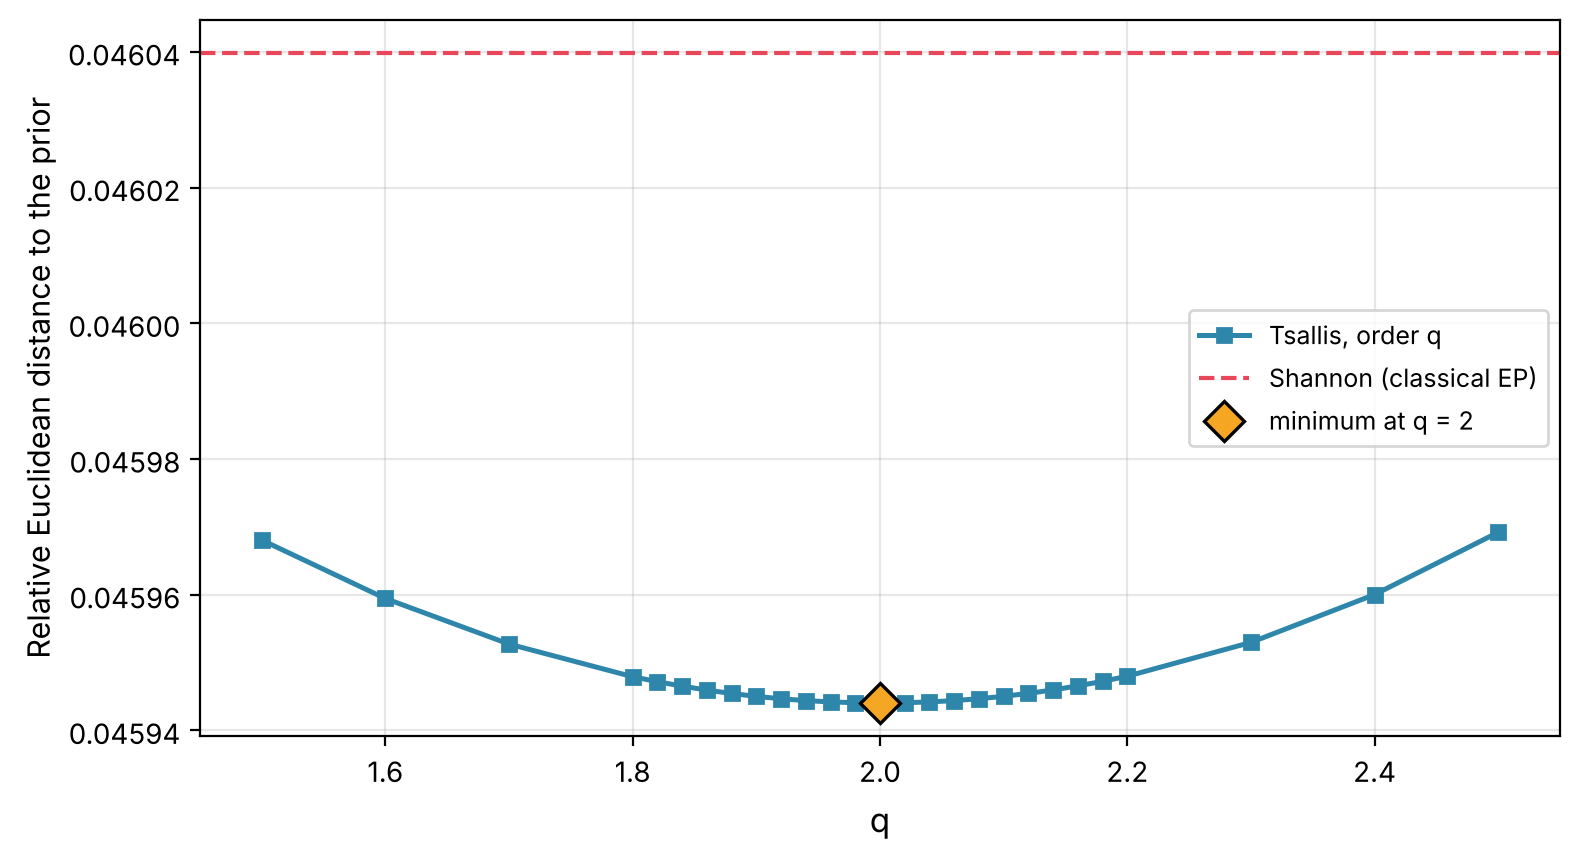
\includegraphics[width=.7\textwidth]{figs/optimal_q_zoom_en.png}
\caption{Relative Euclidean distance between the posterior and the prior,
$\norm{\pt_{q,c} - \p}_2/\norm{\p}_2$, as a function of the order $q$
(database of \citealp{Meucci2008}, $10^5$ scenarios, one inequality view,
$c=0.5$). The dashed line is classical EP. The minimum at $q=2$ follows
from Proposition~\ref{prop:hill}.}
\label{fig:qsweep}
\end{figure}

\begin{table}[t]
\centering
\small
\caption{Relative Euclidean distance between posterior and prior:
Python and GNU Octave implementations (database of \citealp{Meucci2008},
$10^5$ scenarios, one inequality view, $c=0.5$). The Octave values are those
recorded in the repository.}
\label{tab:octave}
\begin{tabular}{lcccccc}
\toprule
 & Shannon & $q=1.5$ & $q=1.9$ & $q=2.0$ & $q=2.1$ & $q=2.5$ \\
\midrule
Octave & 0.046042 & 0.045968 & 0.045945 & 0.045944 & 0.045945 & 0.045969 \\
Python & 0.046040 & 0.045968 & 0.045945 & 0.045944 & 0.045945 & 0.045969 \\
\bottomrule
\end{tabular}

\end{table}

\subsection{A stress experiment}\label{sec:separation}

Outside the cases of Propositions~\ref{prop:local}
and~\ref{prop:jeffrey}, the one of practical interest is a view that asks
for a large change in a moment. This
section measures that case on the equity panel of
Section~\ref{sec:empirical}: $J = \nJ$ daily scenarios for $N = \nN$
stocks, uniform prior and full confidence. A single inequality view
requires the expected return of one stock (CEPU) to exceed its sample mean
by $k$ standard errors,
$\E[X_i] \ge \hat\mu_i + k\,\hat\sigma_i/\sqrt{J}$, for $k$ between 0 and
50. One standard error is \nSEday\% per day, about \nSEann{} percentage
points per year, so the grid goes far beyond any view that a portfolio manager would hold
about an expected return: $k=5$ adds \nExFive{} percentage points per year
to the historical mean and $k=50$ adds \nExFifty. Views of this size appear
in stress testing, where the question is what the scenarios look like if
the market moves to an extreme regime, and the experiment should be read in
that light.

For each $k$ the Shannon and $q=2$ posteriors and the corresponding
mean--variance portfolios are computed (long-only, 30\% cap, risk aversion $2.5$).
Table~\ref{tab:stress} and Figure~\ref{fig:stress} report the effective
numbers of scenarios of orders 2 and 1 as fractions of $J$, the number of
scenarios with zero probability under $q=2$, the 5\% conditional
value-at-risk of the stressed stock under each posterior, and the $\ell_1$
distance between the two portfolios.

\begin{table}[t]
\centering
\footnotesize
\caption{Stress experiment: one inequality view on the expected return of
one stock, $k$ standard errors above its sample mean ($J = \nJ$, uniform
prior, full confidence). $\Delta\mu$ is the corresponding excess over the
historical mean in percentage points per year. $N_2/J$ and $N_1/J$ are the
effective numbers of scenarios of orders 2 (Kish) and 1 (entropy) as
fractions of $J$. EP is the classical (Shannon) posterior. ``Zeros'' is the number of
scenarios with zero probability under $q=2$. CVaR is the 5\% conditional
value-at-risk of the stock, that is, its mean return over the worst 5\% of
probability mass, in per cent per day ($\nCVaRprior$ under the prior).
$\norm{\Delta w}_1$ is the $\ell_1$ distance between the mean--variance
portfolios of the two posteriors. Last row: ranking of the \nN{} stocks in
the reverse order of their sample means.}
\label{tab:stress}
\begin{tabular}{rrccccrccc}
\toprule
 & & \multicolumn{2}{c}{$N_2/J$} & \multicolumn{2}{c}{$N_1/J$} & & \multicolumn{2}{c}{CVaR} & \\
\cmidrule(lr){3-4}\cmidrule(lr){5-6}\cmidrule(lr){8-9}
$k$ & $\Delta\mu$ & EP & $q=2$ & EP & $q=2$ & Zeros & EP & $q=2$ & $\norm{\Delta w}_1$ \\
\midrule
0 & 0 & 1.000 & 1.000 & 1.000 & 1.000 & 0 & $-7.91$ & $-7.91$ & 0.00 \\
1 & 22 & 0.999 & 0.999 & 1.000 & 1.000 & 0 & $-7.66$ & $-7.64$ & 0.02 \\
2 & 44 & 0.998 & 0.998 & 0.999 & 0.999 & 0 & $-7.44$ & $-7.37$ & 0.08 \\
5 & 110 & 0.987 & 0.987 & 0.993 & 0.993 & 1 & $-6.90$ & $-6.67$ & 0.08 \\
10 & 220 & 0.944 & 0.948 & 0.974 & 0.972 & 2 & $-6.25$ & $-5.66$ & 0.07 \\
20 & 439 & 0.755 & 0.815 & 0.903 & 0.884 & 39 & $-5.38$ & $-3.86$ & 0.29 \\
35 & 769 & 0.328 & 0.568 & 0.753 & 0.670 & 296 & $-4.59$ & $-1.71$ & 0.69 \\
50 & 1098 & 0.116 & 0.361 & 0.595 & 0.449 & 734 & $-4.11$ & $0.05$ & 1.18 \\
\midrule
ranking & -- & 0.998 & 0.998 & 0.999 & 0.999 & 0 & -- & -- & 0.00 \\
\bottomrule
\end{tabular}

\end{table}

\begin{figure}[t]
\centering
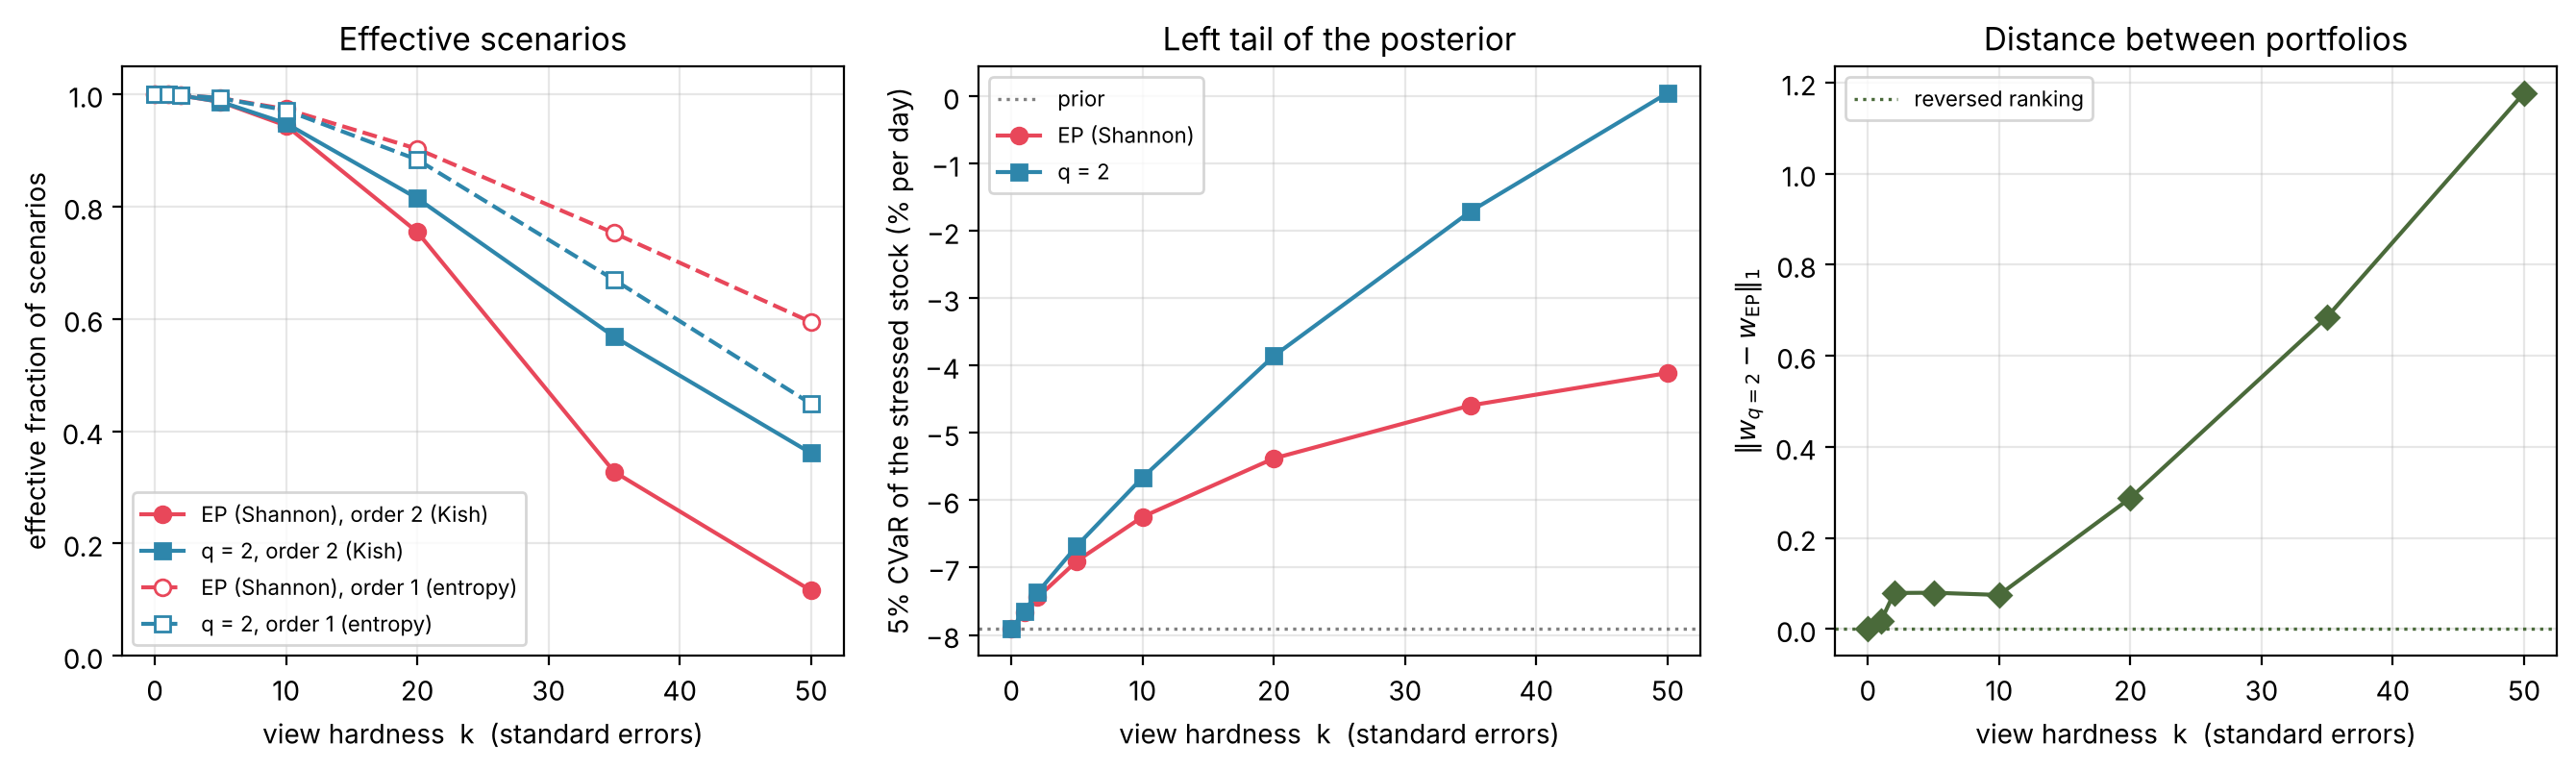
\includegraphics[width=\textwidth]{figs/qep_vs_ep_stress_en.png}
\caption{Stress experiment of Table~\ref{tab:stress}. Left: effective
numbers of scenarios of orders 2 and 1, as fractions of $J$. Centre: 5\%
conditional value-at-risk of the stressed stock under each posterior.
Right: $\ell_1$ distance between the mean--variance portfolios; the dotted
line is the reversed ranking.}
\label{fig:stress}
\end{figure}

Up to $k=5$ the two posteriors are the same for
practical purposes, as Proposition~\ref{prop:local} predicts; the
difference between them grows with $k^2$ for small $k$. The portfolios
differ somewhat earlier ($\norm{\Delta w}_1 = \nDwFive$ at $k=5$) because
the mean--variance step amplifies small differences in expected returns.
From $k=5$ on the stressed stock is at the 30\% cap in both portfolios, and
the distance between them reflects how the rest is allocated.

For larger $k$ the posteriors separate, and each is better by its own
measure, as Proposition~\ref{prop:hill} states. At $k=20$ the Kish
effective number is \nKishTTwenty{} of $J$ for $q=2$ and \nKishSTwenty{}
for Shannon; at $k=50$ it is \nKishTFifty{} against \nKishSFifty. The
entropy-based number goes the other way: \nEnsSFifty{} for Shannon and
\nEnsTFifty{} for $q=2$ at $k=50$. The reason is in the shape of the tilt.
The exponential tilt of Shannon gives very large weights to the few days
with the highest returns of the stock: the most heavily weighted scenario
has \nMaxSTwenty{} times the uniform weight at $k=20$ and \nMaxSFifty{}
times at $k=50$. The truncated linear tilt of $q=2$ limits those weights
to \nMaxTTwenty{} and \nMaxTFifty{} times the uniform weight and obtains
the rest of the required mean by removing scenarios.

That removal is the cost of $q=2$. At $k=20$ it gives zero probability
to \nZerosTwenty{} scenarios and at $k=50$ to \nZerosFifty{} of the \nJ;
these are the days with the lowest returns of the stressed stock. The left tail
of the posterior shrinks accordingly: the 5\% CVaR of the stock, which is
$\nCVaRprior$\% per day under the prior, becomes $\nCVaRSTwenty$\% under
Shannon and $\nCVaRTTwenty$\% under $q=2$ at $k=20$, and $\nCVaRSFifty$\%
against $\nCVaRTFifty$\% at $k=50$. A risk measure computed on the $q=2$
posterior of a strongly bullish view therefore understates the downside
relative to classical EP, which never excludes a scenario. For a strongly
bearish view the truncation removes the best days instead.

The argument for order 2 after Proposition~\ref{prop:hill} was that
posterior moments are estimated with less sampling variance.
Table~\ref{tab:boot} checks it with a bootstrap. The scenarios are
resampled with replacement \nBootReps{} times; in each resample both posteriors are computed for the
same view, and the posterior mean and volatility of the equally weighted
portfolio of the \nN{} stocks are recorded. For mild views the dispersion
of these moments across resamples is nearly the same under both posteriors. For
demanding views it is much lower under $q=2$: at $k=20$ the standard
deviation of the posterior mean is \nBootSdTTwenty{} basis points per day
against \nBootSdSTwenty{} under Shannon, and at $k=50$ it is
\nBootSdTFifty{} against \nBootSdSFifty. The concentration of the Shannon
posterior on the largest observations is related to the finding of
\citet{DeyJuneja2012} that the Kullback--Leibler solution may fail to
exist when the prior has fat tails, and the lower sampling error of the
$\chi^2$ member agrees with what \citet{MakamMillossovichTsanakas2021}
report for stressed simulation models.

\begin{table}[t]
\centering
\small
\caption{Sampling variability of posterior moments in the stress
experiment. Standard deviation, across \nBootReps{} bootstrap resamples of
the scenarios, of the posterior mean of the equally weighted portfolio
(basis points per day), and coefficient of variation of its posterior
volatility, for the view of Table~\ref{tab:stress} at each $k$.}
\label{tab:boot}
\begin{tabular}{rcccc}
\toprule
 & \multicolumn{2}{c}{SD of the posterior mean (bp)} & \multicolumn{2}{c}{CV of the posterior volatility} \\
\cmidrule(lr){2-3}\cmidrule(lr){4-5}
$k$ & EP & $q=2$ & EP & $q=2$ \\
\midrule
0 & 4.9 & 4.9 & 0.050 & 0.050 \\
5 & 3.8 & 3.7 & 0.050 & 0.045 \\
10 & 4.4 & 4.0 & 0.079 & 0.061 \\
20 & 8.3 & 4.8 & 0.163 & 0.093 \\
35 & 21.7 & 6.9 & 0.273 & 0.142 \\
50 & 42.5 & 10.2 & 0.346 & 0.194 \\
\bottomrule
\end{tabular}

\end{table}

Two other designs were tried. A ranking of the \nN{} stocks in
the reverse order of their sample means, which imposes 19 inequalities at
once, moves the posterior very little (Kish effective number \nRankEss{} of $J$
under both posteriors, $\norm{\Delta w}_1 = \nRankDw$), because the differences
between daily mean returns are small relative to their sampling error: the
number of views is not what makes a view set demanding. And a view that
multiplies the volatility of the stock by two or three, leaving its mean
unchanged, separates the family much less than a view on the mean with a
similar loss of effective sample (Kish effective number \nVolKishTTwo{} for $q=2$
against \nVolKishSTwo{} for Shannon for a factor of two, \nVolKishTThree{} against
\nVolKishSThree{} for a factor of three), with no scenario set to zero.
Views on the probability of a tail give identical posteriors for both
members, as Proposition~\ref{prop:jeffrey} implies for a view on a single
event. The pattern of the effective numbers, the zeros and the CVaR in
Table~\ref{tab:stress} is the same when another stock is stressed and for
$q = 1.5$ and $q = 3$; the distance between the portfolios varies with the
stock, because it also depends on where the cap binds. Those results are in
the repository.

% ---------------------------------------------------------------------
\section{View specification}\label{sec:views}
% ---------------------------------------------------------------------

The implementation has one language for views, which is translated into the
inputs of each model: the triple $(P, Q, \Omega)$ of Black--Litterman (BL)
and the constraints~\eqref{eq:constraints} of EP. Table~\ref{tab:views}
lists the types.

\begin{table}[t]
\centering
\small
\caption{Types of views and their form in each model.}
\label{tab:views}
\begin{tabular}{lll}
\toprule
View & Constraint on the posterior (EP) & Black--Litterman \\
\midrule
absolute & $\E[X_i] = \mu^\ast$ & yes \\
relative & $\E[X_i - X_k] = s^\ast$ & yes \\
ranking & $\E[X_{i_1}] \ge \E[X_{i_2}] \ge \dots$ & relative views with $s^\ast \approx 0$ \\
inequality (absolute or relative) & $\E[\cdot] \ge$ or $\le$ a bound & no \\
volatility & $\E[X_i^2] = \sigma^{\ast 2} + \mu_{prior}^2$, or a bound & no \\
tail & $\Pr(X_i < t) \le \pi$ or $\Pr(X_i > t) \le \pi$ & no \\
\bottomrule
\end{tabular}
\end{table}

Two differences matter when the models are compared. BL has no
inequalities: a ranking enters as a chain of relative views with a spread
close to zero, which says that the expected returns are almost equal, with
an uncertainty $\Omega$; EP imposes the one-sided constraint. And views on
volatilities or tails have no counterpart in BL. The uncertainty of the BL
views is set from the stated confidence $c_k$ in view $k$ as
$\Omega_k = \frac{1-c_k}{c_k}\,\tau\, P_k \Sigma P_k^\top$, a closed-form
version of the calibration by confidence levels of \citet{Idzorek2007}.

% ---------------------------------------------------------------------
\section{Application: Argentine equities}\label{sec:empirical}
% ---------------------------------------------------------------------

\subsection{Data and priors}

The universe is the 20 stocks of the leading panel (\emph{panel l\'ider})
of the Buenos Aires stock exchange. The estimation sample consists of daily simple returns in pesos from
24~November~2017 to 22~September~2025, which gives $J = \nJ$ scenarios;
the prior is uniform. The benchmark is a portfolio of these 20 stocks with the
weights of the Merval index at its September 2025 rebalancing, held without
further rebalancing; it is not the index itself. Portfolios
are formed at the close of 22~September~2025. Three missing prices of one
stock (VALO) are filled by linear interpolation; with them the panel is
complete, and the covariance matrix is the sample covariance.

Two priors are used, with the same scenarios and different expected
returns. The \emph{historical} prior is the set of scenarios as observed,
so that prior expected returns are sample means. The \emph{equilibrium}
prior shifts the scenarios so that their means are the returns implied by
the benchmark, $\Pi = \delta\,\Sigma\, w_{bench}$, with $\delta = 2.5$:
each scenario is replaced by $X_j - \hat\mu + \Pi$, which keeps the
covariances and the higher moments. BL uses the equilibrium prior by
construction, with $\tau = 0.05$; with the calibration of $\Omega$ used
here, which is proportional to $\tau$, the BL expected returns do not
depend on that value.

The two priors disagree about expected returns. The historical means are
similar across stocks (between \nMuHistMin\% and \nMuHistMax\% per year in
nominal pesos), while the equilibrium returns are proportional to the
covariance with the benchmark: they are between \nPiLowMin\% and
\nPiLowMax\% for ALUA, VALO and BYMA and between \nPiBankMin\% and
\nPiBankMax\% for the four banks. With the historical prior a
mean--variance investor therefore prefers the stocks with a low covariance
with the benchmark, and with the equilibrium prior the investor holds the benchmark.

\subsection{Views}

The views are based on the opinions that a portfolio manager of Argentine
equities held in September 2025 and shared with the author: (i) within the
energy sector,
the ranking YPFD $\succ$ PAMP $\succ$ TGSU2 $\succ$ CEPU, with confidence
$0.70$; and (ii) each of the two preferred energy stocks (YPFD and PAMP)
outperforms each of four banks (GGAL, BBAR, BMA and SUPV), with confidence
$0.50$. Both statements are ordinal. In EP they enter as $3 + 8 = \nIneq$
inequalities between expected returns, imposed as stated. The confidence
attached to each statement is not used in EP; partial confidence enters
once, through the mixture with the prior with $c=0.5$.
In BL the ranking enters as three relative views with a spread close to
zero and the eight statements about banks as relative views with zero
spread, with the stated confidences in $\Omega$. This encoding gives BL no
information about the direction of the views: a relative view with zero
spread says that two expected returns are equal. BL could carry the
direction with a positive spread, but that requires a number that the
manager did not give. The comparison between BL and EP below is therefore
a comparison between two encodings of ordinal statements, and it says
nothing about BL with quantified views. The views were written
into the code after the end of the evaluation period, so the exercise
illustrates the method and is not a test of the manager's forecasts.

With the historical prior only one of the \nIneq{} inequalities binds
(PAMP over TGSU2), and with the equilibrium prior \nActiveEq{} bind, since
equilibrium returns rank the banks above the energy stocks. In both cases
the views are mild in the sense of Section~\ref{sec:optimalq}: before
mixing with the prior, the Kish effective sample size of the EP posterior
is \nEssHist\% of $J$ with the historical prior and \nEssEq\% with the
equilibrium prior,
and no expected return moves by more than \nShiftEq{} percentage points per
year.

\subsection{Portfolios}

For each prior four portfolios are computed with the same mean--variance
step (long-only, risk aversion $\delta = 2.5$, a cap of 30\% per stock):
one without views, and one for each updating rule, BL, EP and EP with
$q = 2$. For the historical prior the BL formula is applied with the
sample means in place of $\Pi$. The BL portfolios use the BL expected
returns with the covariance matrix of the prior, and the EP portfolios use
the means and covariances of the scenarios under the posterior. Without views the equilibrium prior
reproduces the benchmark, so the benchmark is the no-view portfolio of that
prior. Table~\ref{tab:weights} reports the weights. The cap does not bind
in any of them.

\begin{table}[t]
\centering
\footnotesize
\caption{Portfolio weights (\%) at 22~September~2025, by prior and updating
rule. Simple returns, long-only, 30\% cap, $\delta = 2.5$, $\tau = 0.05$,
global confidence $0.5$ for EP. ``No views'' is the mean--variance
portfolio of each prior; for the equilibrium prior it is the benchmark. The
last row is the $\ell_1$ distance to the no-view portfolio of the same
prior.}
\label{tab:weights}
\begin{tabular}{lrrrrrrrr}
\toprule
 & \multicolumn{4}{c}{Equilibrium prior} & \multicolumn{4}{c}{Historical prior} \\
\cmidrule(lr){2-5}\cmidrule(lr){6-9}
 & No views & BL & EP & $q=2$ & No views & BL & EP & $q=2$ \\
\midrule
ALUA & 2.68 & 2.95 & 3.04 & 3.03 & 16.39 & 15.32 & 16.28 & 16.29 \\
BBAR & 5.20 & 0.00 & 2.65 & 2.64 & 0.00 & 0.00 & 0.00 & 0.00 \\
BMA & 8.01 & 0.00 & 1.01 & 1.01 & 0.00 & 0.00 & 0.00 & 0.00 \\
BYMA & 4.72 & 4.45 & 4.40 & 4.41 & 21.50 & 24.28 & 21.63 & 21.63 \\
CEPU & 6.23 & 3.46 & 3.53 & 3.55 & 0.00 & 0.00 & 0.00 & 0.00 \\
COME & 1.36 & 1.22 & 1.34 & 1.34 & 0.00 & 0.00 & 0.00 & 0.00 \\
CRES & 2.68 & 2.72 & 2.87 & 2.86 & 2.15 & 3.11 & 2.21 & 2.22 \\
EDN & 1.23 & 1.05 & 1.07 & 1.09 & 0.00 & 0.00 & 0.00 & 0.00 \\
GGAL & 15.04 & 7.85 & 13.45 & 13.46 & 0.00 & 0.00 & 0.00 & 0.00 \\
LOMA & 3.47 & 3.39 & 3.30 & 3.35 & 0.00 & 0.00 & 0.00 & 0.00 \\
METR & 0.87 & 0.28 & 0.61 & 0.60 & 0.00 & 0.00 & 0.00 & 0.00 \\
PAMP & 14.68 & 27.05 & 23.26 & 23.24 & 0.00 & 11.09 & 7.23 & 7.23 \\
SUPV & 2.74 & 0.00 & 0.00 & 0.00 & 0.00 & 0.00 & 0.00 & 0.00 \\
TECO2 & 2.19 & 2.20 & 2.35 & 2.31 & 0.00 & 0.00 & 0.00 & 0.00 \\
TGNO4 & 1.17 & 1.14 & 1.11 & 1.10 & 0.00 & 0.00 & 0.00 & 0.00 \\
TGSU2 & 5.64 & 10.69 & 8.00 & 8.02 & 18.45 & 4.69 & 11.00 & 11.00 \\
TRAN & 1.23 & 1.28 & 0.93 & 0.95 & 0.00 & 0.71 & 0.00 & 0.00 \\
TXAR & 5.02 & 4.98 & 5.05 & 5.05 & 3.76 & 5.42 & 3.81 & 3.81 \\
VALO & 1.28 & 1.37 & 1.53 & 1.51 & 21.11 & 22.72 & 21.15 & 21.15 \\
YPFD & 14.55 & 23.91 & 20.49 & 20.47 & 16.63 & 12.65 & 16.68 & 16.68 \\
\midrule
$\norm{w - w_{\text{no views}}}_1$ & -- & 0.54 & 0.36 & 0.36 & -- & 0.38 & 0.15 & 0.15 \\
\bottomrule
\end{tabular}

\end{table}

The choice of $q$ does not matter:
the EP and $q=2$ portfolios differ by $\norm{\Delta w}_1 = \nLoneQhist$
with the historical prior and by \nLoneQeq{} with the equilibrium prior,
as expected for mild views. The prior matters most. The two no-view
portfolios are at a distance of \nLonePrior{} from each other, out of a
maximum of 2, because the portfolio of the historical prior is concentrated
in stocks that have small weights in the benchmark. The views move the
portfolio by less: \nLoneEPhist{} for EP and \nLoneBLhist{} for BL with the
historical prior, \nLoneEPeq{} and \nLoneBLeq{} with the equilibrium
prior. With both priors BL moves the portfolio further than EP, and with the
equilibrium prior it removes three of the four banks. The difference comes
from how confidence enters. BL treats the eleven statements as separate
pieces of evidence, each with its own confidence, and each of them pulls a
spread towards zero; EP imposes the inequalities and is then mixed once
with the prior, which leaves the expected returns about halfway. With
$c=1$ in EP the order is reversed with the equilibrium prior: EP moves the
portfolio by \nLoneEPeqFull{} and BL by \nLoneBLeq{}
(Appendix~\ref{app:robust}).

\subsection{Out-of-sample evaluation}

The portfolios are held from the close of 22~September~2025 to
20~March~2026, \nDays{} trading days after the end of the estimation
sample, without rebalancing. Table~\ref{tab:oos} reports the results and
Figure~\ref{fig:oos} the paths. Returns are nominal, in pesos, and the
Sharpe ratio is computed with a zero risk-free rate; with the peso interest
rates of the period its level is overstated for all the portfolios, and
only comparisons between them are meaningful.

\begin{table}[t]
\centering
\footnotesize
\caption{Out-of-sample results, 22~September~2025 to 20~March~2026
(\nDays{} trading days), buy and hold. Return is the cumulative return over the window, in pesos;
volatility
annualized with 252 days; Sharpe ratio with a zero risk-free rate; tracking
error (TE) and beta relative to the benchmark; DD is drawdown. The last
column is the difference in Sharpe ratio with the no-view portfolio of the
same prior and its 95\% confidence interval from a circular block bootstrap
(blocks of 5 days, 10,000 replications). The minimum-variance portfolio
is computed with the same constraints and is at the 30\% cap in one
stock.}
\label{tab:oos}
\begin{tabular}{lrrrrrrl}
\toprule
 & Return & Vol. & Sharpe & Max.\ DD & TE & Beta & $\Delta$ Sharpe \\
 & (\%) & (\%) & & (\%) & (\%) & & [95\% interval] \\
\midrule
\multicolumn{8}{l}{\emph{Equilibrium prior}} \\
\quad No views (benchmark) & 49.0 & 47.6 & 1.97 & $-21.1$ & -- & -- & -- \\
\quad BL & 48.1 & 40.8 & 2.20 & $-16.7$ & 10.4 & 0.84 & $+0.23$ $[-0.38,\, +0.99]$ \\
\quad EP & 47.6 & 42.8 & 2.10 & $-18.3$ & 6.9 & 0.89 & $+0.13$ $[-0.26,\, +0.59]$ \\
\quad EP, $q=2$ & 47.6 & 42.8 & 2.10 & $-18.3$ & 6.9 & 0.89 & $+0.13$ $[-0.26,\, +0.59]$ \\
\addlinespace
\multicolumn{8}{l}{\emph{Historical prior}} \\
\quad No views & 67.9 & 36.0 & 3.18 & $-17.4$ & 20.9 & 0.69 & -- \\
\quad BL & 68.7 & 35.5 & 3.24 & $-17.2$ & 22.8 & 0.66 & $+0.06$ $[-0.26,\, +0.35]$ \\
\quad EP & 67.2 & 35.5 & 3.19 & $-17.5$ & 21.5 & 0.68 & $+0.02$ $[-0.13,\, +0.14]$ \\
\quad EP, $q=2$ & 67.2 & 35.5 & 3.19 & $-17.5$ & 21.5 & 0.68 & $+0.02$ $[-0.13,\, +0.14]$ \\
\addlinespace
\multicolumn{8}{l}{\emph{Reference portfolios}} \\
\quad Equally weighted & 53.8 & 49.7 & 2.04 & $-21.8$ & 8.5 & 1.03 & -- \\
\quad Minimum variance & 62.7 & 38.7 & 2.81 & $-21.3$ & 23.1 & 0.71 & -- \\
\bottomrule
\end{tabular}

\end{table}

\begin{figure}[t]
\centering
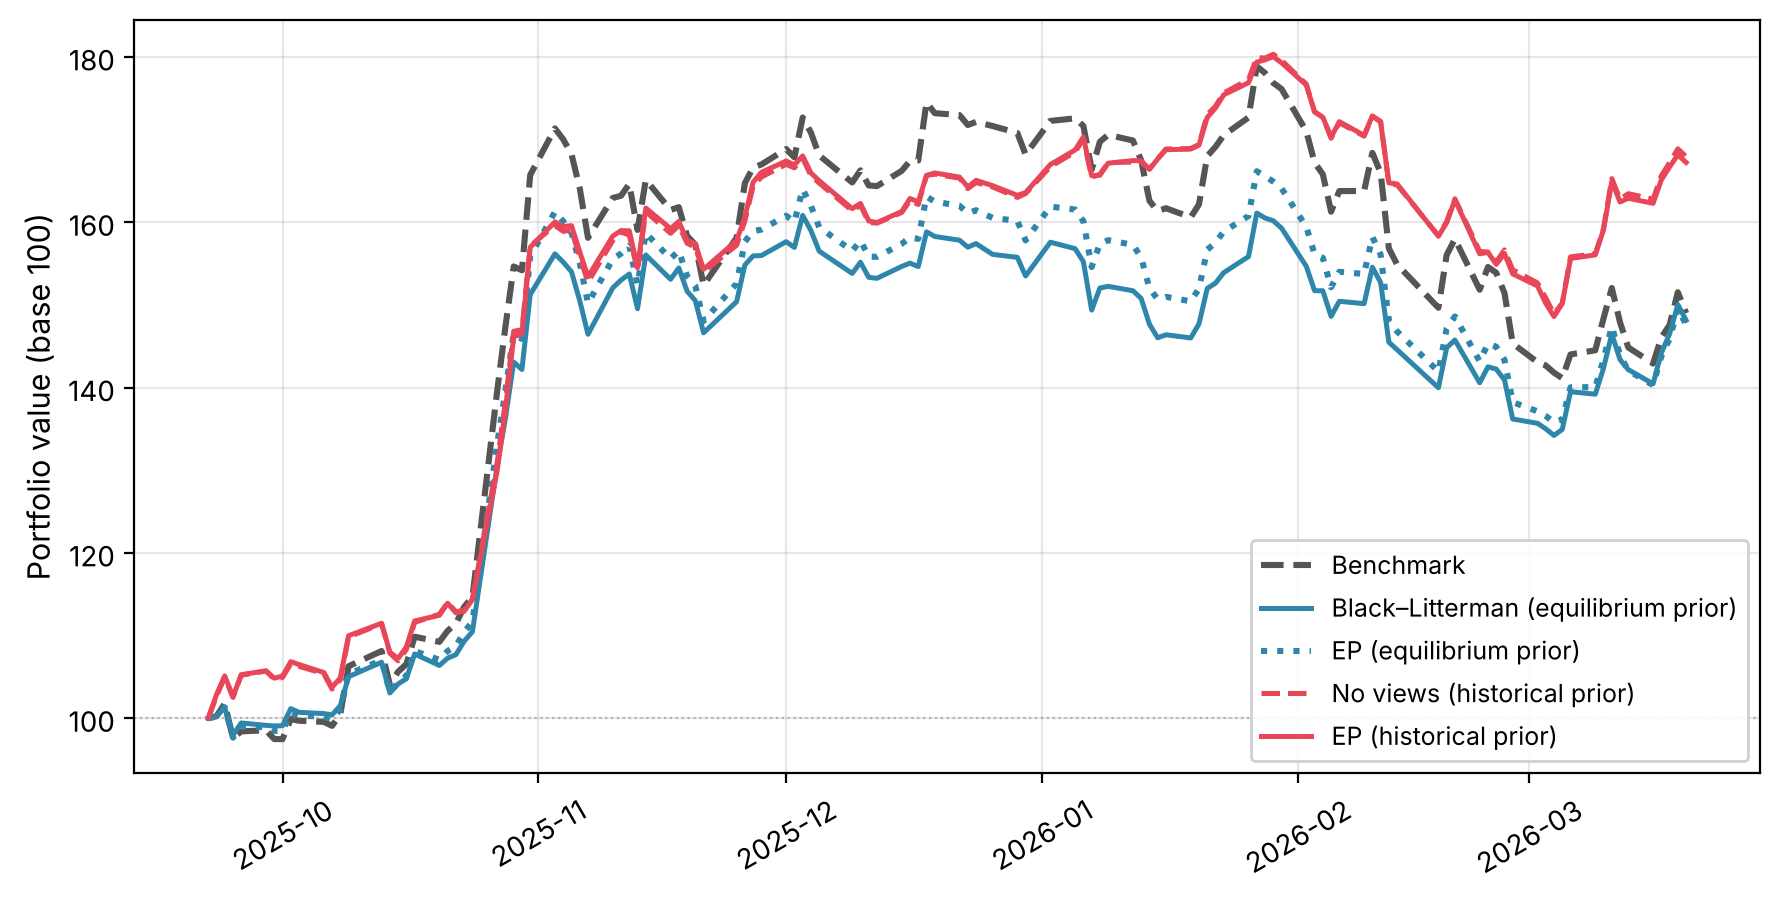
\includegraphics[width=.85\textwidth]{figs/oos_evolution_en.png}
\caption{Value of the portfolios, 22~September~2025 to 20~March~2026 (base
100, buy and hold). The $q=2$ portfolios coincide with the EP portfolios
and are omitted, as are BL with the historical prior and the two reference
portfolios; with the historical prior the EP and no-view portfolios are
almost indistinguishable.}
\label{fig:oos}
\end{figure}

The portfolios fall into two groups according to the prior. Those built on
the equilibrium prior behave like the benchmark: cumulative returns between
\nRetEPeq\% and \nRetBench\% and Sharpe ratios between \nShBench{} and
\nShBL. Those built on the historical prior return between \nRetEP\% and
\nRetBLhist\% with about three quarters of the volatility of the
benchmark, and their
Sharpe ratios are between \nShMVhist{} and \nShBLhist. The no-view
portfolio already has a Sharpe ratio of \nShMVhist. Low-volatility
stocks did well in the period: the minimum-variance portfolio, which uses
no expected returns, has a Sharpe ratio of \nShMinVar{} and the equally
weighted portfolio one of \nShEW. Two stocks on which the manager expressed
no view, VALO and BYMA, add \nContribTop{} percentage points to the return
of the no-view portfolio of the historical prior relative to the
benchmark, more than the whole difference of \nContribTotal{} points
between the two.

Within each prior the views add little. With the historical prior the EP
portfolio has a Sharpe ratio $\nBootEPdiff$ higher than the no-view
portfolio, with a 95\% interval of $[\nBootEPlo, \nBootEPhi]$. With the
equilibrium prior BL improves on the benchmark by $\nBootBLdiff$
($[\nBootBLlo, \nBootBLhi]$) and EP by $\nBootEPeqdiff$
($[\nBootEPeqlo, \nBootEPeqhi]$), in both cases with lower volatility and
a slightly lower return. None of these differences can be distinguished
from zero with \nDays{} observations. The difference between the two
no-view portfolios is larger, $\nBootPriordiff$ in Sharpe ratio, but it is
at the margin of what the window can detect. Its interval is
$[\nBootPriorlo, \nBootPriorhi]$ with blocks of five days, and with blocks
of 1, 3, 5, 10 and 20 days and ten other bootstrap seeds for each length
the lower end lies between
$\nBootPriorLoMin$ and $\nBootPriorLoMax$. Ten intervals were computed in
all, with no adjustment for multiple comparisons. BL and EP are closer to
each other within a prior than either is to its counterpart with the other
prior.

A direct comparison of BL on the equilibrium prior with EP on historical
scenarios, which is how the two methods are usually run, would show EP
ahead by $\nBootUsualdiff$ in Sharpe ratio (\nShEP{} against \nShBL, with
an interval of $[\nBootUsuallo, \nBootUsualhi]$). The design decomposes
that gap: $\nBootPriordiff$ is the difference between the two no-view
portfolios, and the effects of the views within each prior
($\nBootEPdiff$ for EP and $\nBootBLdiff$ for BL) account for the rest.
The BL formula applied to the historical prior does as
well as EP, and EP applied to the equilibrium prior does no better than
BL. Given the encoding of the views, in which BL shrinks spreads towards
zero and carries no direction, this compares two encodings in one window
and does not rank the two rules.

\subsection{Limitations and robustness}\label{sec:limitations}

The evaluation covers one window of six months in one market, so it
describes an episode. The window was not chosen in advance, the views were
written into the code after it, and the period includes the legislative
election of October 2025. One day carries much of the level of the Sharpe
ratios: on \nExtDay, the first session after the election, the benchmark
gained \nExtBench\% and the no-view portfolio of the historical prior
\nExtMVhist\%. Without that day their Sharpe ratios are \nShBenchEx{} and
\nShMVhistEx; the order of the two priors does not depend on it. The good performance of the historical prior is
the performance of a few stocks with a low covariance with the benchmark
in that episode, and it depends on the estimation sample: with the
scenarios of the last five or three years instead of the whole sample, the
no-view portfolio of the historical prior has a Sharpe ratio between
\nShWinNVmin{} and \nShWinNVmax, close to that of the benchmark.

A placebo confirms that the window carries little information about the
views. Replacing them by their opposite (the reverse ranking, and banks
above energy stocks) leaves the Sharpe ratios of the BL portfolios unchanged to two decimals,
because a ranking written as spreads close to zero has no direction, and
gives EP portfolios with Sharpe ratios of \nShPlaceboEP{} with the
historical prior and \nShPlaceboEPeq{} with the equilibrium prior, against
\nShEP{} and \nShEPeq{} with the manager's views. With the equilibrium
prior the opposite views already hold under the prior, so that portfolio is
the benchmark.

Transaction costs are ignored. Moving from the benchmark to the EP
portfolio with the historical prior requires trading \nTurnEP{} of the
portfolio value, counting purchases and sales; at 50 basis points per side
this costs about \nCostEP\% once, which is small relative to the
differences in Table~\ref{tab:oos}. With a risk-free rate of 30\% per year
instead of zero the Sharpe ratios of all the portfolios fall, to
\nShBenchRf{} for the benchmark and \nShMVhistRf{} for the no-view
portfolio of the historical prior, and the order of the eight portfolios
of the design does not change.

Three features of the data qualify the performance of the historical
prior. The universe is the set of stocks in the index at the formation
date, so the historical means are those of stocks selected at the end of
the sample. The three stocks that carry \nWIlliq\% of the no-view portfolio
(VALO, BYMA and ALUA) have a zero return on between \nZeroIlliqMin\% and
\nZeroIlliqMax\% of the days of the estimation sample, against
\nZeroLiqMin\% to \nZeroLiqMax\% for YPFD and the four banks. Infrequent
trading lowers measured covariances, which is what the optimizer rewards
under that prior, and the cost assumed above does not include the price
impact of positions of that size. And the returns are nominal, in pesos,
over a sample with high and variable inflation; no variant in dollars or
in real terms was run.

Appendix~\ref{app:robust} reports the variants above and others that change
one assumption at a time: the confidence, the order $q$, the cap, the risk
aversion, log instead of simple returns, daily rebalancing instead of buy
and hold, and the encoding of the views about banks as equalities with
targets halfway to the prior, which was the first version of this
exercise. With the historical prior, the Sharpe ratio of EP differs from that of
its no-view portfolio by between $\nRobMin$ and $\nRobMax$ in every
variant, and the EP and $q=2$ portfolios differ by less than \nRobQmax{}
in $\ell_1$ distance. With the equilibrium prior the ranges are wider: EP
exceeds the benchmark by between zero and $\nRobEqMax$, the maximum with
full confidence, and the two EP portfolios differ by less than
\nRobQmaxEq. The
encoding with equalities has no solution with the equilibrium prior,
because the equalities for the two energy stocks imply, by subtraction,
that the difference between the expected returns of YPFD and PAMP is half
its prior value, which contradicts the ranking when the prior
ranks PAMP first.

% ---------------------------------------------------------------------
\section{Extension to fixed income}\label{sec:bonds}
% ---------------------------------------------------------------------

For bonds the natural invariant is the change in yield, $\Delta y$, and
not the price return, whose distribution changes as the bond approaches
maturity. The repository includes a version of the pipeline that runs EP on
scenarios of yield changes and optimizes on the price returns that they
imply. This section describes it; no empirical results for bonds are
reported in this paper.

With modified duration $D_t$ and convexity $C_t$, the price return is
approximated by
\begin{equation}\label{eq:duration}
\frac{\Delta P_t}{P_{t}} \;\approx\; -\,D_{t}\,\Delta y_t \;+\; \tfrac{1}{2}\,C_{t}\,(\Delta y_t)^2,
\end{equation}
with three options: a constant duration (that of the formation date), a
duration that changes with time, and the latter with the convexity term.
The mapping gives the price return only; the carry is not included.
Views are stated on $\Delta y$ with the types of Table~\ref{tab:views}. A
view that the yield of bond $i$ will fall by more than that of bond $k$ is
$\E[\Delta y_i] \le \E[\Delta y_k]$, so a ranking of bonds by expected
performance has the reverse order when it is written in terms of yields.
With different durations the order of yield changes is not the order of
price returns, and a view about relative performance is better written on
the mapped price returns, which are also functions of the scenarios. A tail
view bounds the probability of a large rise in yield,
$\Pr(\Delta y_i > t) \le \pi$.

Panels of emerging-market sovereign bonds are often unbalanced, because
bonds issued recently have short histories. For such panels the repository
includes an estimator of the covariance matrix that works pair by pair on
the dates on which both series are observed, with a minimum number of
observations, and makes the result positive semidefinite, when necessary,
with the alternating projections of \citet{Higham2002}; the scenarios for
EP are then the dates on which all the series are observed. No result of
this paper depends on it: the equity panel of
Section~\ref{sec:empirical} is complete.

% ---------------------------------------------------------------------
\section{Conclusion}\label{sec:conclusion}
% ---------------------------------------------------------------------

Entropy Pooling can be run with any member of the Tsallis family at the
cost of solving a dual problem with one variable per view. With a uniform
prior each member maximizes the effective number of scenarios of its own
order. Classical EP maximizes the entropy-based number and keeps every
scenario; $q=2$ maximizes the effective sample size of Kish, which
governs the sampling variance of posterior moments, and is the Euclidean
projection of the prior onto the set of distributions that satisfy the
views.

For most views the choice is of no consequence. The members of the family
agree to first order in the size of the views and give identical posteriors
for views on the probability of an event. They differ for views that
require a large change in a moment, as in stress testing, and there the
choice is a trade-off: $q=2$ avoids the concentration of the posterior on a
few extreme scenarios, and it does so by excluding the scenarios that
contradict the view, which reduces the tail risk that the posterior shows.
Which of the two is preferable depends on whether the posterior will be
used to estimate moments or to measure risk.

In the application to Argentine equities the views of a practitioner are
mild, the two versions of EP give the same portfolio, and the out-of-sample
gap between EP and Black--Litterman is the gap between their priors, in a
window too short to establish any of the differences statistically. A
comparison of Black--Litterman with Entropy Pooling in which each method
has its usual prior also measures the difference between the priors, and a
design that holds the prior fixed is needed to separate the two. Two extensions are left for future
work: an evaluation over many formation dates with views recorded in
advance, and the fixed-income application.

% ---------------------------------------------------------------------
\section*{Declarations}
% ---------------------------------------------------------------------

\paragraph{Funding.} This research received no external funding.

\paragraph{Competing interests.} The author works in the asset management
industry. The opinions expressed are his own and do not represent those of
his employer. Pablo J.~Escapa shared the equity views in a personal
capacity and took no part in the analysis.

\paragraph{Data and code availability.} The code that produces every table
and figure is available at
\begin{center}
\url{https://github.com/rodrigocorvalan93/non_extensive_q_entropy_pooling}
\end{center}
and the README maps each result to its script. The commit history dates
the framework, its implementations in Octave and Python, the search over
$q$ and the application to the Merval to March 2026. The scenario database of
Section~\ref{sec:numerics} is the one distributed with
\citet{Meucci2008}. The daily prices of the stocks and the weights of the
benchmark are from Bloomberg, and their redistribution is subject to its
licence terms. The repository documents the format of the input files and
includes the output of every step, from which the tables are generated
without the price data.

\paragraph{Disclaimer.} This paper is academic research. It is not
investment advice or an offer to buy or sell any security. The portfolios
reported illustrate a method and are not recommendations, and the
out-of-sample results cover a single window and are no guide to future
performance.

% ---------------------------------------------------------------------
\appendix
\section{Dual derivations}\label{app:dual}
% ---------------------------------------------------------------------

\paragraph{Shannon.} The Lagrangian of~\eqref{eq:primal} with $D = D_{KL}$ is
\[
L = \sum_j x_j(\ln x_j - \ln p_j) + \boldsymbol{\lambda}^\top(A\x - \mathbf{b})
+ \boldsymbol{\nu}^\top(A_{eq}\x - \mathbf{b}_{eq}),
\qquad \boldsymbol{\lambda} \ge 0 .
\]
Its derivative with respect to $x_j$ is $\ln x_j - \ln p_j + 1 + z_j$, with
$\mathbf{z} = A^\top\boldsymbol{\lambda} + A_{eq}^\top\boldsymbol{\nu}$.
Setting it to zero gives~\eqref{eq:kkt-shannon}. The solution is positive,
so the constraint $x_j \ge 0$ is never active.

\paragraph{Tsallis, $q>1$.} With $D = D_q$,
$\partial L/\partial x_j = \frac{q}{q-1}\,(x_j/p_j)^{q-1} + z_j$. If
$z_j < 0$ the derivative vanishes at
$(x_j/p_j)^{q-1} = -\frac{q-1}{q}\,z_j > 0$, which is the interior solution
in~\eqref{eq:kkt-tsallis}. If $z_j \ge 0$ the derivative is positive for
every $x_j > 0$, so the minimum of $L$ over $x_j \ge 0$ is at $x_j = 0$.
The two cases together give~\eqref{eq:kkt-tsallis}. For $0<q<1$ the
derivative tends to $-\infty$ as $x_j \to 0$, so the minimum is interior
and requires $z_j > 0$:
$x_j = p_j\,[(1-q)\,z_j/q]^{-1/(1-q)}$, with no truncation.

\paragraph{Dual function.} Let
$\x(\boldsymbol{\lambda},\boldsymbol{\nu})$ be the minimizer of $L$ over
$\x \ge 0$. The dual function
$g(\boldsymbol{\lambda},\boldsymbol{\nu}) = L\big(\x(\boldsymbol{\lambda},\boldsymbol{\nu}),
\boldsymbol{\lambda},\boldsymbol{\nu}\big)$ is concave, as a pointwise minimum of
functions that are affine in the multipliers, and its gradient is
$\big(A\x - \mathbf{b},\; A_{eq}\x - \mathbf{b}_{eq}\big)$ evaluated at
$\x(\boldsymbol{\lambda},\boldsymbol{\nu})$. At a maximum of $g$ subject to
$\boldsymbol{\lambda} \ge 0$ the equality constraints hold, the inequality
constraints hold, and $\lambda_i (A\x - \mathbf{b})_i = 0$ for each
inequality, so $\x(\boldsymbol{\lambda},\boldsymbol{\nu})$ satisfies the
optimality conditions of~\eqref{eq:primal} and is the posterior.

% ---------------------------------------------------------------------
\section{Proofs and further properties of the family}\label{app:proofs}
% ---------------------------------------------------------------------

\paragraph{Proof of Proposition~\ref{prop:local}.} For $\x$ close to $\p$
the non-negativity constraints are not active, and the optimality
conditions are $\varphi'(x_j/p_j) + z_j = 0$ with
$\mathbf{z} = A_{eq}^\top \boldsymbol{\nu}$, together with the views. Since
$\varphi''(1) > 0$, $\varphi'$ has a differentiable inverse $\psi$ near
$\varphi'(1)$, with $\psi'(\varphi'(1)) = 1/\varphi''(1)$, and
$x_j = p_j\,\psi(-z_j)$. At $\varepsilon = 0$ the solution is $\x = \p$,
with $z_j = -\varphi'(1)$ for all $j$; this is
$\mathbf{z} = A_{eq}^\top \boldsymbol{\nu}^0$ for the vector
$\boldsymbol{\nu}^0$ that has $-\varphi'(1)$ in the position of the
normalization row and zeros elsewhere. Let
$G(\boldsymbol{\nu}, \varepsilon) = A_{eq}\,\x(\boldsymbol{\nu}) -
A_{eq}\p - \varepsilon\,\mathbf{d}$. Then $G(\boldsymbol{\nu}^0, 0) = 0$
and
$\partial G/\partial \boldsymbol{\nu} = -\,A_{eq} P A_{eq}^\top /
\varphi''(1)$ at $(\boldsymbol{\nu}^0, 0)$, which is non-singular because
$A_{eq}$ has full row rank. By the implicit function theorem
$\boldsymbol{\nu}(\varepsilon)$ is differentiable at $0$, with
$\boldsymbol{\nu}'(0) = -\varphi''(1)\,(A_{eq} P A_{eq}^\top)^{-1}
\mathbf{d}$, and therefore
$\x'(0) = -P A_{eq}^\top \boldsymbol{\nu}'(0)/\varphi''(1)
= P A_{eq}^\top (A_{eq} P A_{eq}^\top)^{-1}\mathbf{d}$. The problem is
convex, so the point that satisfies the optimality conditions is the
posterior. \qed

If $\varphi$ is three times differentiable the remainder
in~\eqref{eq:linear} is $O(\varepsilon^2)$. In the stress experiment of
Section~\ref{sec:separation}, with an equality view $k$ standard errors
above the mean, the largest difference between the Shannon and $q=2$
posteriors divided by $k^2$ is constant to within 15\% for $k$ between
$0.25$ and $2$.

\paragraph{Proof of Proposition~\ref{prop:jeffrey}.} Let $\x$ satisfy the
views and let $\bar{\x}$ be given by~\eqref{eq:jeffrey}. By Jensen's
inequality applied within each cell with weights $p_j/p(E_k)$,
\[
D_\varphi(\x\|\p) = \sum_k p(E_k) \sum_{j \in E_k} \frac{p_j}{p(E_k)}\,
\varphi\!\Big(\frac{x_j}{p_j}\Big)
\;\ge\; \sum_k p(E_k)\, \varphi\!\Big(\frac{\pi_k}{p(E_k)}\Big)
= D_\varphi(\bar{\x}\|\p),
\]
with equality only if $x_j/p_j$ is constant within each cell, that is, only
if $\x = \bar{\x}$. \qed

\paragraph{R\'enyi divergence.} Let
$t(\x) = \sum_j x_j^{\,q} p_j^{\,1-q}$, so that the Tsallis relative entropy
is $D_q = (t-1)/(q-1)$ and the divergence of \citet{Renyi1961} is
$D^R_q = \ln t/(q-1)$. By Jensen's inequality $t \ge 1$ on the simplex for
$q>1$ and $t \le 1$ for $q<1$, and both divergences are increasing
functions of $t$ in the first case and decreasing functions of $t$ in the
second. They therefore have the same minimizer over $\mathcal{F}$, and the
same holds for any other monotone function of $t$: within this class the
posterior depends on $q$ and not on the function applied to $t$, as
\citet{DeyJuneja2012} note for the polynomial divergence that they use. Using the
R\'enyi divergence instead of the Tsallis relative entropy would give the
same posteriors. With a uniform prior the R\'enyi divergence is related to the effective
numbers of Section~\ref{sec:optimalq} by $N_q(\x) = J\,\exp\!\big(-D^R_q(\x\|\p)\big)$.
As a numerical check, the R\'enyi problem was solved directly in the
probabilities with a general-purpose optimizer on a subsample of 60
scenarios, without using the dual of Section~\ref{sec:dual}; the result
coincides with the Tsallis posterior to within $10^{-8}$ for
$q \in \{1.5,\, 2,\, 2.5\}$.

\paragraph{Limit $q \to 1$.} For fixed $\x$ in the simplex, write
$x_j^{\,q} p_j^{\,1-q} = x_j\, e^{(q-1)\ln(x_j/p_j)}$ and expand the
exponential:
$t(\x) = 1 + (q-1)\sum_j x_j \ln(x_j/p_j) + O\big((q-1)^2\big)$. Hence
$(t-1)/(q-1) \to D_{KL}(\x\|\p)$, and $\ln t/(q-1)$ has the same limit.
Section~\ref{sec:numerics} reports how the posteriors approach the Shannon
posterior.

% ---------------------------------------------------------------------
\section{Robustness of the application}\label{app:robust}
% ---------------------------------------------------------------------

Table~\ref{tab:robust} repeats the exercise of
Section~\ref{sec:empirical} changing one assumption at a time.

\begin{table}[h]
\centering
\footnotesize
\caption{Robustness of the application. Out-of-sample Sharpe ratios (zero
risk-free rate, except in the last row) of the portfolios of
Table~\ref{tab:oos} under alternative assumptions. The last two columns are $\ell_1$ distances with the
historical prior: between the EP and the no-view portfolios (``views'') and
between the EP and the $q=2$ portfolios (``$q$''); in the rows for
$q = 1.5$ and $q=3$ the column $q$ uses that order. ``Blended equalities''
encodes the views about banks as equalities with targets halfway between
the prior and the view, and then applies the mixture with $c=0.5$ as well;
it has no solution with the equilibrium prior. In the rows for $\delta$ the
same value is used for the equilibrium returns and for the optimizer. The
Sharpe ratio of the benchmark is \nShBench{} with buy and hold and
\nShBenchDaily{} with daily rebalancing.}
\label{tab:robust}
\begin{tabular}{lcccccccc}
\toprule
 & \multicolumn{2}{c}{Equilibrium} & \multicolumn{4}{c}{Historical prior} & \multicolumn{2}{c}{$\norm{\Delta w}_1$} \\
\cmidrule(lr){2-3}\cmidrule(lr){4-7}\cmidrule(lr){8-9}
 & BL & EP & No views & BL & EP & $q$ & views & $q$ \\
\midrule
Base case & 2.20 & 2.10 & 3.18 & 3.24 & 3.19 & 3.19 & 0.15 & 0.0002 \\
Blended equalities & 2.20 & -- & 3.18 & 3.24 & 3.23 & 3.23 & 0.18 & 0.0003 \\
Full confidence, $c=1$ & 2.20 & 2.21 & 3.18 & 3.24 & 3.20 & 3.20 & 0.31 & 0.0004 \\
$q = 1.5$ & 2.20 & 2.10 & 3.18 & 3.24 & 3.19 & 3.19 & 0.15 & 0.0001 \\
$q = 3$ & 2.20 & 2.10 & 3.18 & 3.24 & 3.19 & 3.19 & 0.15 & 0.0004 \\
Cap 20\% & 2.17 & 2.10 & 3.13 & 3.14 & 3.14 & 3.14 & 0.15 & 0.0002 \\
Cap 40\% & 2.20 & 2.10 & 3.18 & 3.24 & 3.19 & 3.19 & 0.15 & 0.0002 \\
No cap & 2.20 & 2.10 & 3.18 & 3.24 & 3.19 & 3.19 & 0.15 & 0.0002 \\
$\delta = 1$ & 2.20 & 2.10 & 2.71 & 2.71 & 2.65 & 2.65 & 0.11 & 0.0004 \\
$\delta = 5$ & 2.20 & 2.09 & 3.24 & 3.21 & 3.24 & 3.24 & 0.08 & 0.0001 \\
Log returns & 2.25 & 2.13 & 3.39 & 3.43 & 3.41 & 3.41 & 0.09 & 0.0002 \\
Estimation sample: last 5 years & 1.99 & 2.04 & 2.15 & 2.05 & 2.15 & 2.16 & 0.09 & 0.0001 \\
Estimation sample: last 3 years & 2.04 & 2.06 & 2.07 & 2.01 & 2.12 & 2.12 & 0.11 & 0.0007 \\
Reversed views (placebo) & 2.20 & 1.97 & 3.18 & 3.24 & 3.24 & 3.24 & 0.22 & 0.0021 \\
Daily rebalancing & 2.26 & 2.17 & 3.19 & 3.26 & 3.21 & 3.21 & 0.15 & 0.0002 \\
Risk-free rate of 30\% & 1.56 & 1.48 & 2.45 & 2.50 & 2.45 & 2.45 & 0.15 & 0.0002 \\
\bottomrule
\end{tabular}

\end{table}

% ---------------------------------------------------------------------
\begin{thebibliography}{99}
\bibitem[Almeida and Garcia(2012)]{AlmeidaGarcia2012}
Almeida, C., and R.~Garcia (2012): ``Assessing Misspecified Asset Pricing
Models with Empirical Likelihood Estimators,'' \textit{Journal of
Econometrics}, 170(2), 519--537.

\bibitem[Antoine et~al.(2007)Antoine, Bonnal, and Renault]{AntoineBonnalRenault2007}
Antoine, B., H.~Bonnal, and E.~Renault (2007): ``On the Efficient Use of the
Informational Content of Estimating Equations: Implied Probabilities and
Euclidean Empirical Likelihood,'' \textit{Journal of Econometrics}, 138(2),
461--487.

\bibitem[Avellaneda et~al.(2001)Avellaneda, Buff, Friedman, Grandchamp, Kruk, and Newman]{AvellanedaEtAl2001}
Avellaneda, M., R.~Buff, C.~Friedman, N.~Grandchamp, L.~Kruk, and J.~Newman
(2001): ``Weighted Monte Carlo: A New Technique for Calibrating Asset-Pricing
Models,'' \textit{International Journal of Theoretical and Applied Finance},
4(1), 91--119.

\bibitem[Black and Litterman(1992)]{BlackLitterman1992}
Black, F., and R.~Litterman (1992): ``Global Portfolio Optimization,''
\textit{Financial Analysts Journal}, 48(5), 28--43.

\bibitem[Borland(2002)]{Borland2002}
Borland, L. (2002): ``A Theory of Non-Gaussian Option Pricing,''
\textit{Quantitative Finance}, 2(6), 415--431.

\bibitem[Borland et~al.(1998)Borland, Plastino, and Tsallis]{BorlandPlastinoTsallis1998}
Borland, L., A.~R. Plastino, and C.~Tsallis (1998): ``Information Gain within
Nonextensive Thermostatistics,'' \textit{Journal of Mathematical Physics},
39(12), 6490--6501.

\bibitem[Borwein and Lewis(1991)]{BorweinLewis1991}
Borwein, J.~M., and A.~S. Lewis (1991): ``Duality Relationships for
Entropy-Like Minimization Problems,'' \textit{SIAM Journal on Control and
Optimization}, 29(2), 325--338.

\bibitem[Cressie and Read(1984)]{CressieRead1984}
Cressie, N., and T.~R.~C. Read (1984): ``Multinomial Goodness-of-Fit
Tests,'' \textit{Journal of the Royal Statistical Society, Series B},
46(3), 440--464.

\bibitem[Csisz\'ar(1975)]{Csiszar1975}
Csisz\'ar, I. (1975): ``$I$-Divergence Geometry of Probability
Distributions and Minimization Problems,'' \textit{Annals of Probability},
3(1), 146--158.

\bibitem[Csisz\'ar(1991)]{Csiszar1991}
Csisz\'ar, I. (1991): ``Why Least Squares and Maximum Entropy? An Axiomatic
Approach to Inference for Linear Inverse Problems,'' \textit{Annals of
Statistics}, 19(4), 2032--2066.

\bibitem[Deville and S\"arndal(1992)]{DevilleSarndal1992}
Deville, J.-C., and C.-E. S\"arndal (1992): ``Calibration Estimators in
Survey Sampling,'' \textit{Journal of the American Statistical
Association}, 87(418), 376--382.

\bibitem[Dey and Juneja(2012)]{DeyJuneja2012}
Dey, S., and S.~Juneja (2012): ``Incorporating Fat Tails in Financial Models
Using Entropic Divergence Measures,'' arXiv:1203.0643. Earlier version:
``Entropy Approach to Incorporate Fat Tailed Constraints in Financial
Models,'' SSRN Working Paper 1647048 (2010).

\bibitem[Diaconis and Zabell(1982)]{DiaconisZabell1982}
Diaconis, P., and S.~L. Zabell (1982): ``Updating Subjective
Probability,'' \textit{Journal of the American Statistical Association},
77(380), 822--830.

\bibitem[Glasserman and Xu(2014)]{GlassermanXu2014}
Glasserman, P., and X.~Xu (2014): ``Robust Risk Measurement and Model Risk,''
\textit{Quantitative Finance}, 14(1), 29--58.

\bibitem[Glasserman and Yu(2005)]{GlassermanYu2005}
Glasserman, P., and B.~Yu (2005): ``Large Sample Properties of Weighted Monte
Carlo Estimators,'' \textit{Operations Research}, 53(2), 298--312.

\bibitem[He and Litterman(1999)]{HeLitterman2002}
He, G., and R.~Litterman (1999): ``The Intuition Behind Black--Litterman
Model Portfolios,'' Investment Management Research, Goldman, Sachs \& Co.,
December. Available at SSRN 334304.

\bibitem[Higham(2002)]{Higham2002}
Higham, N.~J. (2002): ``Computing the Nearest Correlation Matrix---A
Problem from Finance,'' \textit{IMA Journal of Numerical Analysis}, 22(3),
329--343.

\bibitem[Hill(1973)]{Hill1973}
Hill, M.~O. (1973): ``Diversity and Evenness: A Unifying Notation and Its
Consequences,'' \textit{Ecology}, 54(2), 427--432.

\bibitem[Idzorek(2007)]{Idzorek2007}
Idzorek, T. (2007): ``A Step-by-Step Guide to the Black--Litterman Model: Incorporating
User-Specified Confidence Levels,''
in \textit{Forecasting Expected Returns in the Financial Markets}, ed.\ by
S.~Satchell. Academic Press, 17--38.

\bibitem[Imbens et~al.(1998)Imbens, Spady, and Johnson]{ImbensSpadyJohnson1998}
Imbens, G.~W., R.~H. Spady, and P.~Johnson (1998): ``Information Theoretic
Approaches to Inference in Moment Condition Models,'' \textit{Econometrica},
66(2), 333--357.

\bibitem[Jizba and Korbel(2019)]{JizbaKorbel2019}
Jizba, P., and J.~Korbel (2019): ``Maximum Entropy Principle in Statistical
Inference: Case for Non-Shannonian Entropies,'' \textit{Physical Review
Letters}, 122, 120601.

\bibitem[Kish(1965)]{Kish1965}
Kish, L. (1965): \textit{Survey Sampling}. John Wiley \& Sons, New York.

\bibitem[Kitamura and Stutzer(1997)]{KitamuraStutzer1997}
Kitamura, Y., and M.~Stutzer (1997): ``An Information-Theoretic Alternative to
Generalized Method of Moments Estimation,'' \textit{Econometrica}, 65(4),
861--874.

\bibitem[Kong et~al.(1994)Kong, Liu, and Wong]{KongLiuWong1994}
Kong, A., J.~S. Liu, and W.~H. Wong (1994): ``Sequential Imputations and
Bayesian Missing Data Problems,'' \textit{Journal of the American
Statistical Association}, 89(425), 278--288.

\bibitem[Kullback(1959)]{Kullback1959}
Kullback, S. (1959): \textit{Information Theory and Statistics}. John
Wiley \& Sons, New York.

\bibitem[Makam et~al.(2021)Makam, Millossovich, and Tsanakas]{MakamMillossovichTsanakas2021}
Makam, V.~D., P.~Millossovich, and A.~Tsanakas (2021): ``Sensitivity Analysis
with $\chi^2$-Divergences,'' \textit{Insurance: Mathematics and Economics},
100, 372--383.

\bibitem[Meucci(2008)]{Meucci2008}
Meucci, A. (2008): ``Fully Flexible Views: Theory and Practice,''
\textit{Risk}, 21(10), 97--102.

\bibitem[Meucci(2012)]{Meucci2012}
Meucci, A. (2012): ``Effective Number of Scenarios in Fully Flexible
Probabilities,'' \textit{GARP Risk Professional}, February, 32--35.

\bibitem[Newey and Smith(2004)]{NeweySmith2004}
Newey, W.~K., and R.~J. Smith (2004): ``Higher Order Properties of GMM and
Generalized Empirical Likelihood Estimators,'' \textit{Econometrica},
72(1), 219--255.

\bibitem[P\'ezier(2007)]{Pezier2007}
P\'ezier, J. (2007): ``Global Portfolio Optimization Revisited: A Least
Discrimination Alternative to Black--Litterman,'' ICMA Centre Discussion
Papers in Finance DP2007-07, University of Reading.

\bibitem[Press\'e et~al.(2013)Press\'e, Ghosh, Lee, and Dill]{PresseEtAl2013}
Press\'e, S., K.~Ghosh, J.~Lee, and K.~A. Dill (2013): ``Nonadditive Entropies
Yield Probability Distributions with Biases Not Warranted by the Data,''
\textit{Physical Review Letters}, 111, 180604.

\bibitem[R\'enyi(1961)]{Renyi1961}
R\'enyi, A. (1961): ``On Measures of Entropy and Information,'' in
\textit{Proceedings of the Fourth Berkeley Symposium on Mathematical
Statistics and Probability}, Vol.~1, 547--561. University of California Press, Berkeley.

\bibitem[Shore and Johnson(1980)]{ShoreJohnson1980}
Shore, J.~E., and R.~W. Johnson (1980): ``Axiomatic Derivation of the
Principle of Maximum Entropy and the Principle of Minimum Cross-Entropy,''
\textit{IEEE Transactions on Information Theory}, 26(1), 26--37.

\bibitem[Stutzer(1996)]{Stutzer1996}
Stutzer, M. (1996): ``A Simple Nonparametric Approach to Derivative Security
Valuation,'' \textit{Journal of Finance}, 51(5), 1633--1652.

\bibitem[Tsallis(1988)]{Tsallis1988}
Tsallis, C. (1988): ``Possible Generalization of Boltzmann--Gibbs
Statistics,'' \textit{Journal of Statistical Physics}, 52(1--2), 479--487.

\bibitem[Tsallis(2009)]{Tsallis2009}
Tsallis, C. (2009): \textit{Introduction to Nonextensive Statistical
Mechanics: Approaching a Complex World}. Springer, New York.

\bibitem[Tsallis(2015)]{Tsallis2015}
Tsallis, C. (2015): ``Conceptual Inadequacy of the Shore and Johnson Axioms
for Wide Classes of Complex Systems,'' \textit{Entropy}, 17(5), 2853--2861.

\bibitem[Tsallis et~al.(2003)Tsallis, Anteneodo, Borland, and Osorio]{TsallisEtAl2003}
Tsallis, C., C.~Anteneodo, L.~Borland, and R.~Osorio (2003): ``Nonextensive
Statistical Mechanics and Economics,'' \textit{Physica A}, 324(1--2), 89--100.

\bibitem[Zubizarreta(2015)]{Zubizarreta2015}
Zubizarreta, J.~R. (2015): ``Stable Weights that Balance Covariates for
Estimation with Incomplete Outcome Data,'' \textit{Journal of the American
Statistical Association}, 110(511), 910--922.
\end{thebibliography}

\end{document}
